% Williams Physics Thesis template
% Patterned after the work of Cole Meisenhelder '15
% Commented by Prof. Charlie Doret, 12/2016

\documentclass[12pt, oneside]{book} 

% The \usepackage{} command will import predefined fonts, symbols, environments, etc.  For example, the ams packages below come from the American Mathematical Society and include all kinds of useful math symbols like integrals
\usepackage{amscd}
\usepackage{amsmath}
\usepackage{amssymb}
\usepackage{amsthm}
\usepackage{verbatim}
\usepackage[utf8]{inputenc}
\usepackage{geometry}                		% See geometry.pdf to learn the layout options. There are lots.
\geometry{letterpaper}                   		% ... or a4paper or a5paper or ... 
%\geometry{landscape}                		% Activate for for rotated page geometry
\usepackage[pdftex]{graphicx}				% Use pdf, png, jpg, or eps� with pdflatex; use eps in DVI mode	
\usepackage{setspace}
\usepackage{physics}
\usepackage{subcaption}
\usepackage[numbers]{natbib}
\usepackage{pdfpages}
\usepackage{bm}
\usepackage{wrapfig}				% enables the use of \wrapfig, for figures with text wrapped around them
%\usepackage{lipsum}			% gives access to \lipsum, which dumps some latin text into your document as filler if you want to check formatting

%\usepackage[parfill]{parskip}    		% Activate to begin paragraphs with an empty line rather than an indent



% Here we set the page dimensions to match the standard thesis format.  These values should not be changed.
%%% SET LENTGH AND WIDTH %%%
\setlength{\textwidth}{6.5in}
\setlength{\textheight}{8.5in}
\setlength{\oddsidemargin}{0pt}
\setlength{\evensidemargin}{0pt}
\setlength{\topmargin}{0pt}
\setlength{\marginparsep}{0pt}
\setlength{\marginparwidth}{1in}


%\begin{document} starts LaTeX looking for actual content.  Everything above this point is purely formatting.
\begin{document}

\begin{titlepage}
\begin{center}

% \vspace* creates some vertical white space on the page to make the title page look more pleasing.  \vspace would do much the same thing, but would not insert the white space if we were at the top of a fresh page.  As this is the start of the document we're obviously at the beginning of a page, so the asterisk is necessary to ensure we still put in two cm of white space.
\vspace*{2cm}

{\huge Investigation of Bond Strain Effects on XANES Structure Spectra by Supervised Machine
	Learning} % \huge sets the font size.  Other options include things like \large, \Large, \small, \tiny, etc.

\vspace{2cm}

{\large by\\Jeremy K. Thaller}

\vspace{2cm}
{Professor Anatoly Frenkel, Advisor}

% \vfill creates an arbitrary amount of vertical white space as necessary to fill the page
\vfill

A thesis submitted in partial fulfillment\\
of the requirements for the\\
Erasmus Mundus Joint Master Degrees: \\
Masters in Materials Science Exploring Large Scale Facilities

\vspace*{3cm}

Brookhaven National Labs\\
Brookhaven, New York\\
\today % you might choose to set a permanent date, but \today will put in today's date
\end{center}
\end{titlepage}

% \frontmatter defines the pieces of the thesis which will use roman numerals for page numbering
\frontmatter 


% \chapter{} and/or \chapter*{} will create a chapter in your thesis.  Including the asterisk will cause the chapter to not appear in the table of contents.

% \input will reference a particular .tex file.  Here we are grabbing a file entitled Abstract stored in the folder Chapters
\chapter{Abstract}
% Here is where you'll include the actual text for your abstract.  Because this lives inside the main document and will be included with a \input command, no tags are needed to start a new document.  Instead, just type.


% Your abstract will summarize your thesis in one or two paragraphs.  This brief summary should emphasize methods and results, not introductory material.

% X-ray absorption spectroscopy (XAS) is a widely used experimental technique for material characterization. The two
A recently published method \cite{Timoshenko2017} enables the decoding of X-ray absorption near edge structure (XANES) spectra of nanoparticles to obtain important structural descriptors: coordination numbers and bond distances. Utilizing supervised machine learning (ML), the method trains an artificial neural network (ANN) to recognize a relationship between the nanoparticle structure and the XANES spectrum. Once trained, the ANN is used to ``invert'' an unknown spectrum to obtain the corresponding descriptors of the catalyst structure. Bond strain is known to be an important catalytic descriptor, yet, its accurate determination in reaction conditions is hampered by high temperature and low weight loading of real catalysts. ML–assisted XANES analysis offers a promising new direction for extracting the bond strain information from XANES---and not from extended x-ray absorption fine structure (EXAFS) analysis. Using simulated XANES spectra of Au nanoparticles, we have developed an ANN capable of ``inverting'' an unseen XANES spectrum and predicting structural disorder in the form of mean-squared displacement. The utility of the method was demonstrated on computer-simulated nanoparticles of degrees of disorder. Further work to test the model onto particles of varying sizes and bridge the model's predictive domain onto experimental absorption spectra is required.

% Further, the network is being trained to predict additional disorder descriptors, which would allow for the reconstruction of the radial distribution function, $g(r)$. This prediction is possible in part due to a new statistical averaging approach whereby XANES spectra of disordered structures are created from simulated XANES spectra of non-disordered structures.

% https://www.worldscientific.com/doi/abs/10.1142/9789811204579_0007
% Y. Lin, M. Topsakal, J. Timoshenko, D. Lu, S. Yoo, A. I. Frenkel
% Machine-Learning assisted structure determination of metallic nanoparticles: A benchmark
% In: Handbook on Big Data and Machine Learning in the Physical Sciences, World Scientific Series on Emerging Technologies, v.2, Chapter 7, pp. 127-140 (2020).
\chapter{Executive Summary}
% Here we have your executive summary.

Your executive summary will give a detailed summary of your thesis, hitting the high points and perhaps including a figure or two.  This should have all of the important take-home messages; though details will of course be left for the thesis itself, here you should give enough detail for a reader to have a good idea of the content of the full document.  Importantly, this summary should be able to stand alone, separate from the rest of the document, so although you will be emphasizing the key results of your work, you will probably also want to include a sentence or two of introduction and context for the work you have done.

\begin{figure}[h!]
    \centering
    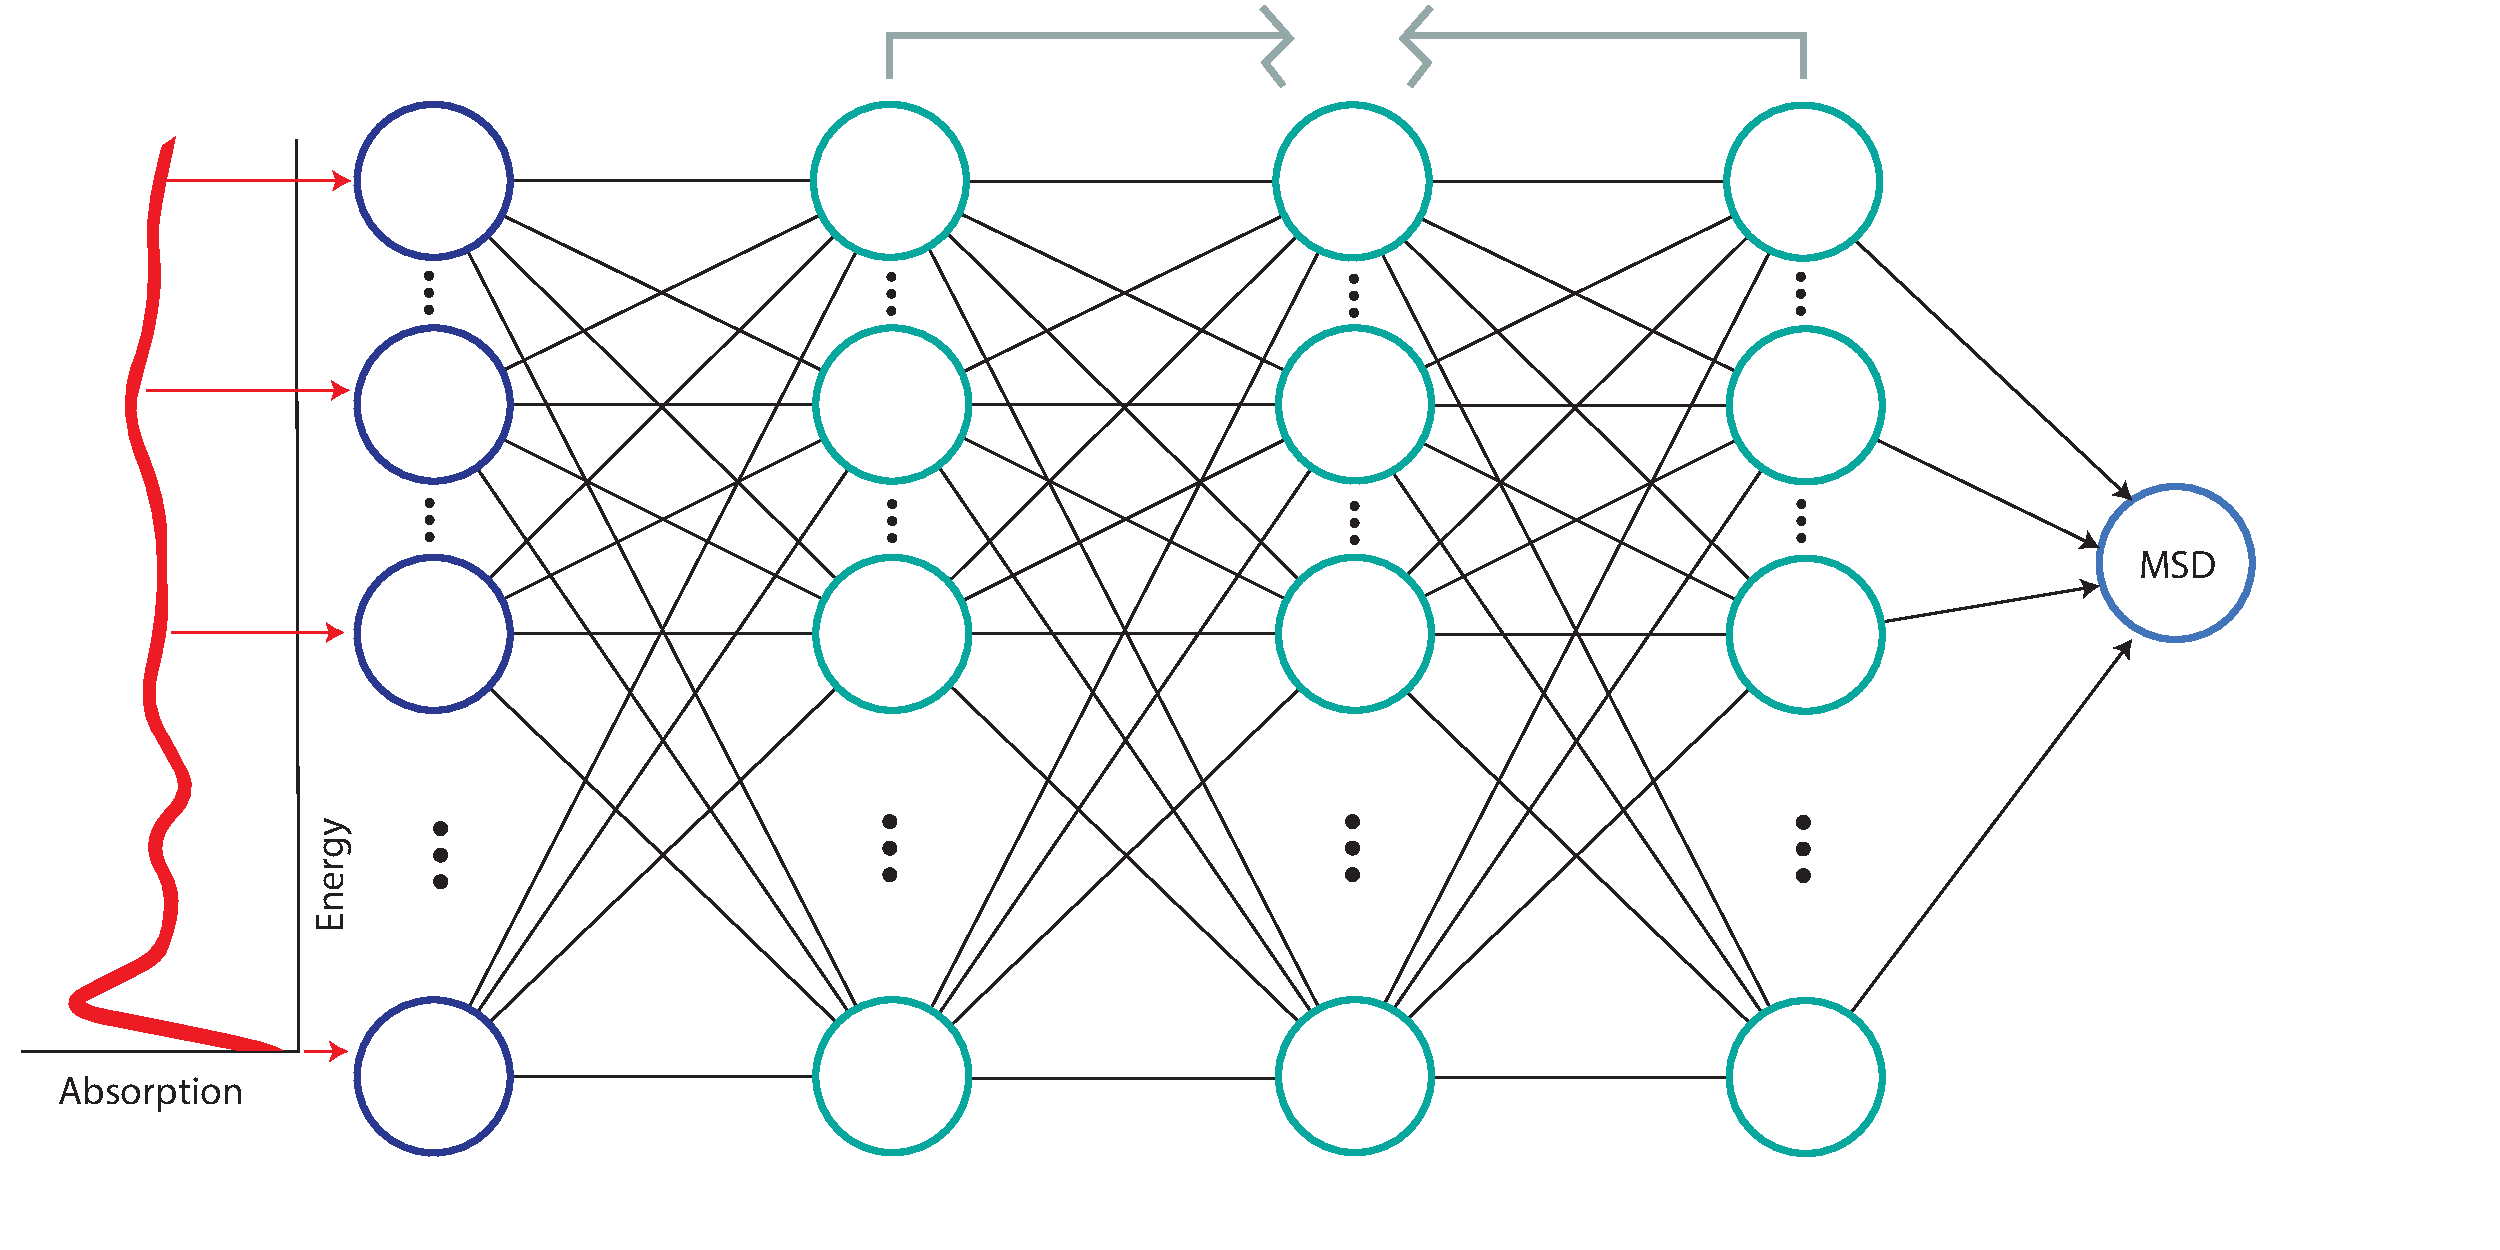
\includegraphics[width=\linewidth]{Chapters/Figures/thesis-design.pdf}
    \caption[Project Approach]{Thesis design}
\end{figure}


\chapter{Acknowledgments}
% Here we have a section where you might choose to acknoweldge your family, fellow students, advisor, dog, etc.

I would like to thank my advisor Professor Anatoly Frenkel and my professors in Germany and Poland over the past two years. I also owe a great debt of gratitude towards those who took the time to help proofread my work, as well as the free and open-source software (FOSS) community.

%\tableofcontents will create a table of contents.  By default it will include entries for any \chapter, \section, and \subsection command that appears in your thesis unless you have called the tag with an asterisk
\tableofcontents

\listoffigures

% \mainmatter defines the main body of the thesis and marks where regular numbering will begin
\mainmatter

\chapter{Introduction}
% Look!  A mock introduction

The introduction is one of the most important pieces of your thesis.  Here is a place for you to introduce the problem(s) on which you have worked and place them in the larger context of your field.  You should aim to ensure that this section is completely understandable to virtually anyone - and certainly anyone with a sophomore-level grasp of physics.  Presumably, this will include references to the literature.

In addition to setting your work into context, a second good idea for your introduction is to give a short outline for what the rest of your thesis will discuss.  This is often done in the closing paragraph(s) of the introduction with sentences like ``In the following chapters \ldots " and ``Chapter 2 discusses \ldots"  Tremendous detail is not required in this outline, but rather just a brief road map for the rest of the document.

\section{X-ray Absorption Spectroscopy}
\emph{I want to describe the problem we're trying to solve in this section. So I want to motivate the problem by describing XAFS a little so I can describe the limitations of XANES and why this project is useful. More in-depth explanations can be placed in chapter 2}

\subsection{EXAFS}
Extended X-ray Absorption Fine Structure (EXAFS)

\subsection{XAFS}
X-ray Absorption Fine-Structure spectroscopy, or XAFS, refers to the study of absorption spectra created from high-intensity x-ray interactions.

Probably want to talk about these papers in this section \cite{timoshenko2018neural} \cite{Timoshenko2017}.



\chapter{A second chapter}
% % Chapter 2: XAFS Simulations
% % Chapter 2: XANES
% \textit{In this section, I can write about XANES to a super in-depth extent, and likely the bulk of this chapter will be about FEFF and FDMNES theoretical calculations}
% \section{Maybe derivation of EXAFS Equation}
% \section{FEFF vs. FDMNES Approaches}
% \section{Theoretical XANES Calculations}
% -------------------------------------------------------------

Before making any predictions, neural networks must first be trained on a large quantity of data. Specifically, to teach our neural network to predict the mean squared displacement (MSD), we must first generate a large quantity of training data comprised of XANES spectra, each labeled with a known MSD. Gathering such a large quantity of high-quality experimental data would be impractically time-intensitive and expensive. Rather, simulations provide a practical alternative, though even simulating each possible disordered structure individually, would be extremely time-intensive. This process is discussed in section \ref{sec:traditional-disorder}. First, a discussion on the development of a new method for simulating disordered nanoparticles is presented in sections \ref{sec:start-disorder}--\ref{sec:end-disorder}. The new process utilizes the statistical averaging of non-disordered structures. Instead of simulating hundreds of defined, disordered structures, we run many XANES simulations of simple, non-disordered structures and generate the disordered spectra via clever statistical averaging. In this chapter, we explain this statistical weighting process in-depth, beginning with the creation of simple, non-disordered spectra for the FEFF input files and culminating in the creation of many possible disordered spectra with known MSDs. The efficacy and limitations of this approach are discussed in section \ref{sec:pa-feff-vs-gaussian-feff}.

\section{Generating Distortion Not Disorder} \label{sec:start-disorder}
Instead of creating structures with a range of \textit{disorder}, we instead begin by generating structures with a range of \textit{distortion}. Wheres \textit{disorder} refers to a statistical average of atomic displacement from their original position, characterized by MSD and the width $ \sigma^2 $ of a partial radial distribution function, \textit{distortion} refers only to isotropic expansion or contraction of the subject. Equivalently, we define distortion as a radial shift in all atomic positions away from (or towards) the center atomic absorber.

% Figure created in distortion-visualizations.ipynb 
\begin{figure}[h]
	\centering
	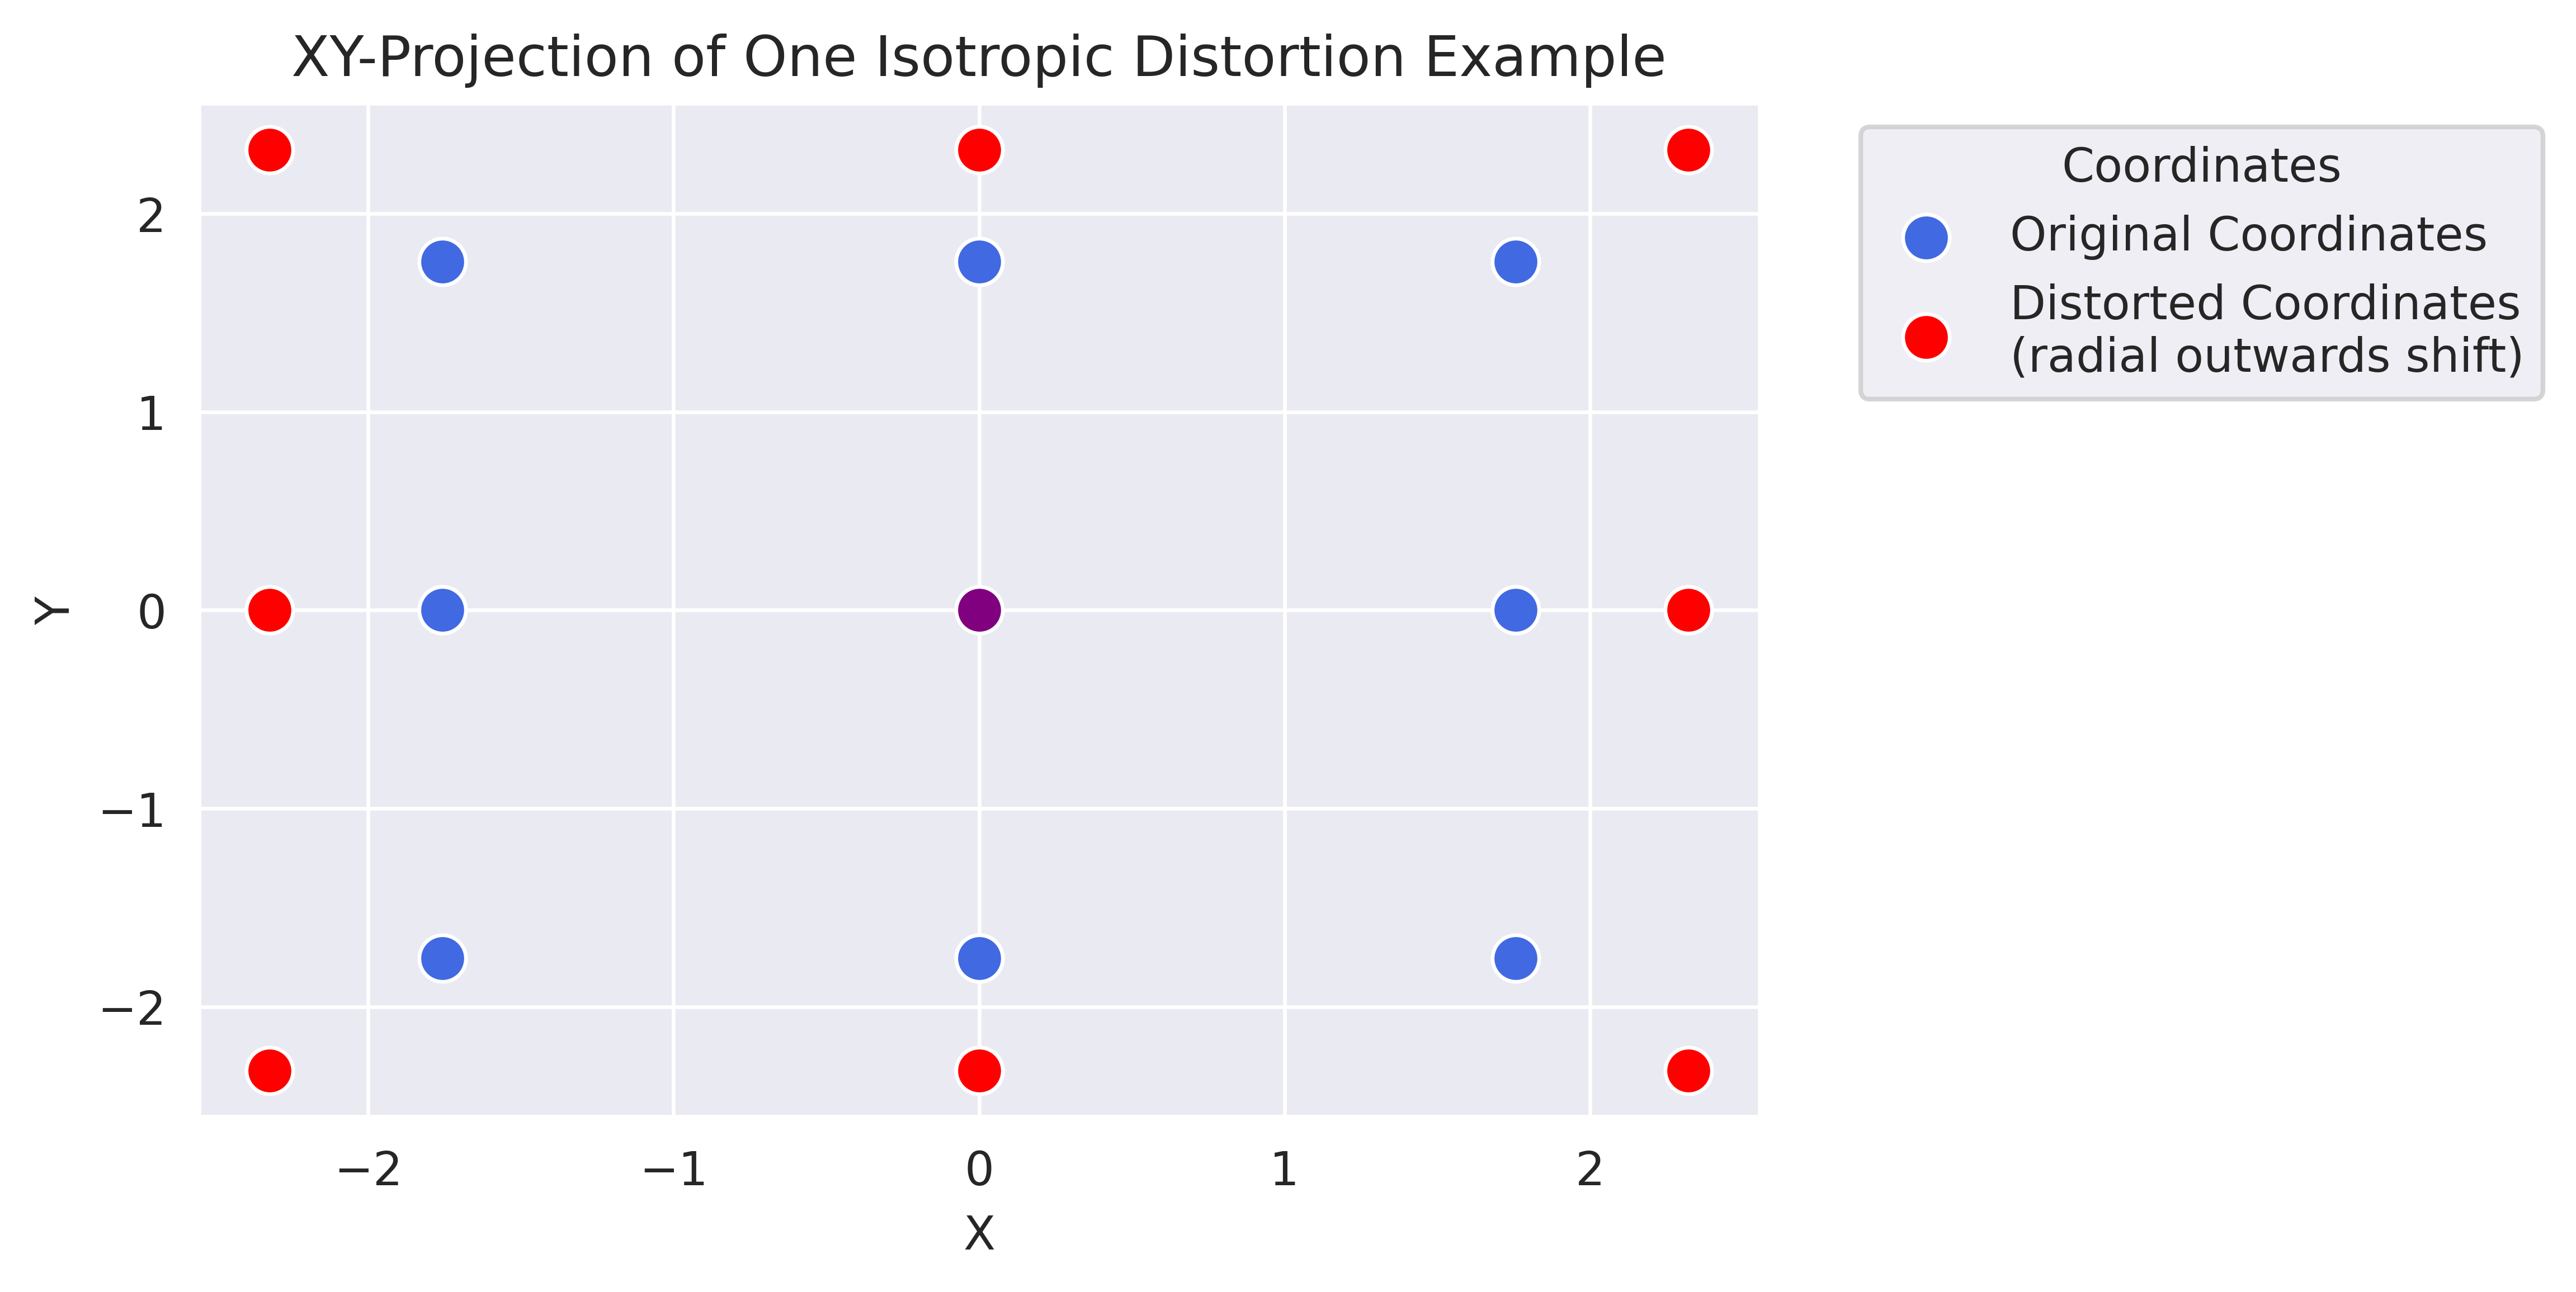
\includegraphics[width=\linewidth]{Chapters/Figures/2d_distortion_example.png}
	\caption[2D Distortion]{Each point represents an atom of first 12 nearest neighbors of a Au cluster projected onto the $xy$\nobreakdash-plane. The four corner points actually represent two atoms because of the projection. The blue atoms represent the original coordinates, and the red atoms represent the radially shifted coordinates. The center absorber atom is purple since its original position is the same as its distorted position.}
	\label{fig:2d-distortion}
\end{figure}

A 2-dimensional projection of this isotropic distortion is presented in Figure \ref{fig:2d-distortion}. Though the figure only shows the $xy$\nobreakdash-plane projection of the first 12 nearest neighbors, the actual structure used consists of the first four shells (561 atoms) with a lattice constant of 4.0782~\AA~to match that of bulk Au.\textit{Citation? Wolfram Element Data?} In reality, the nearest-neighbor distances for Au nanoparticles are likely smaller \textit{gold-lattice-const}; this can be accounted for later on in the averaging process since the original coordinates will only be one structure out of many. The important part is that the crystal structure is correct. 

We generate a total of 91 FEFF input files with different levels of distortion. Each file contains the same center absorber located at $ (0,0,0) $, but all other first shell atomic coordinates are in a shifted location on the range of $ -0.45 $~\AA~to~$ +0.45 $~\AA~in increments of $ 0.01 $~\AA. For example, the FEFF input file with the greatest inward shift has all first nearest neighbor atoms shifted $ 0.45 $~\AA~radially inwards towards the center absorber, and the FEFF input file with the largest outwards shift has the first nearest neighbor coordinates shifted $ 0.45 $~\AA~radially outwards away from the center absorber. The atoms in the outer shells are scaled accordingly to preserve the crystal structure according to:

\begin{equation}
	\label{eq:distortionator}
	\vb*{\rho}_{shifted} = \dfrac{\vb*{\rho} * \vert \vb*{\rho} \vert_{min} + \delta}{\vert \vb*{\rho} \vert_{min}} 
\end{equation}
% alpha = (df[df.rho > 0].rho.min() + delta)/df[df.rho > 0].rho.min()
% df_temp['rho'] *= alpha

\begin{minipage}{\linewidth}
Each FEFF input file is run with the following parameters: 
\begin{Verbatim}[samepage=true, numbers=left]
    SCF 4.6 0 30 .5 1
    EDGE    L3
    EXCHANGE    5   0.2 0.5
    S02 1.
    XANES   3.7 0.05    0.1
    FMS 7

    POTENTIALS
    0	79	Au	-1	-1	0.
    1	79	Au	-1	-1	0.
\end{Verbatim}
~
\end{minipage}

Running the 91 simulations (one for each of the distorted structure) takes approximately 30 minutues. Were we to generate thousands more or employ RMC or MD, this process could take weeks of compute time. We plot the resulting XANES spectra from the FEFF simulations in figure \ref{fig:feff-results}.

\begin{figure}[h]
	\centering
    \makebox[\textwidth][c]{
	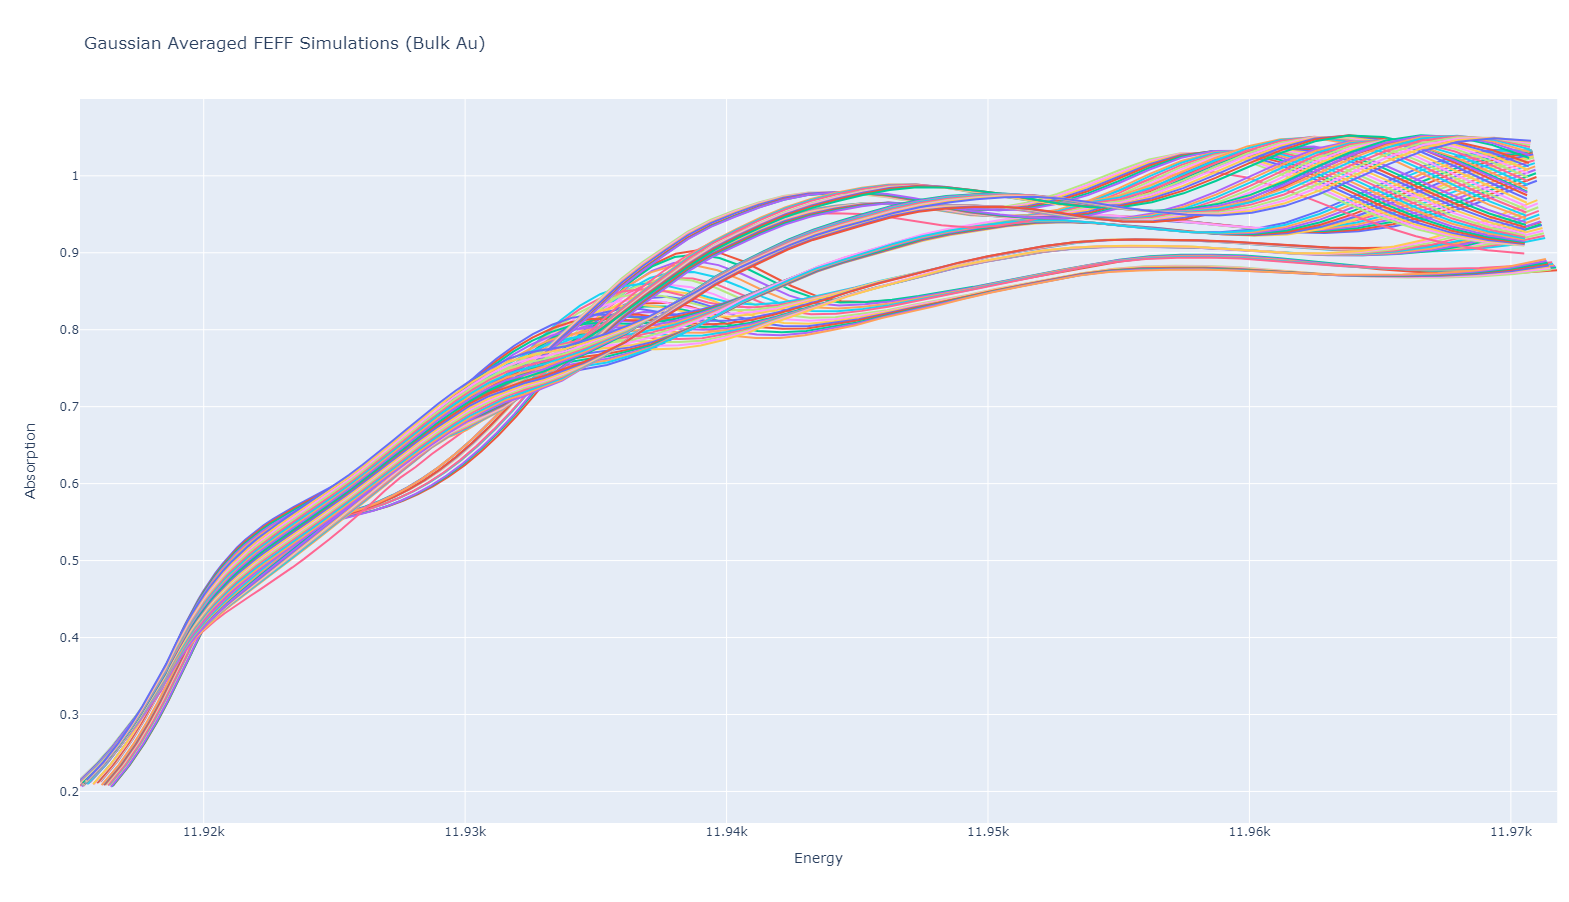
\includegraphics[width=1.1\linewidth]{Chapters/Figures/newplot.png}}
	\caption[FEFF Simulations Results]{\textit{TEMPORARY - way too much info. I'll select a few. }Each spectrum represents the FEFF simulation results for a different distorted structure. For each spectrum, the crystal structure and center absorber remain constant, the only parameter that varies is the euclidean distance from the center to the other coordinates.}
	\label{fig:feff-results}
\end{figure}

\section{Generating Disorder via Probability Distribution Averaging}

One way to characterize system disorder is with the Gaussian width, $ \sigma $ , of the partial radial distribution function. The idea of our statistical averaging method is to emulate this width by weighting the simulated XANES spectra accordingly. For example, Figure \ref{fig:gaussian-weighting-hist} depicts a histogram with $ \sigma=0.1 $~\AA. Each histogram bin represents a simulated XANES spectrum with a different isotropic displacement. For example, the bin at $ \Delta\rho=0.0 $~\AA~represents the simulated XANES spectrum with no distortion, and the bin at $ \Delta\rho=-0.2 $~\AA~represents the simulated XANES spectrum with all the atomic coordinates shifted isotropically inwards towards the center absorber by $ 0.2 $~\AA. The height of each bin, $ f(\Delta\rho) $, represents the relative contribution of each simulated XANES spectrum towards the resulting weighted spectrum. For visual clarity, Figure \ref{fig:gaussian-weighting-hist} depicts only 40 bins; the actual weighting includes 91 bins ranging from $ -0.45 $~\AA~to~$ +0.45 $~\AA.
% figure created in playground.ipynb
% !htb
\begin{figure}[h!]
	\centering
	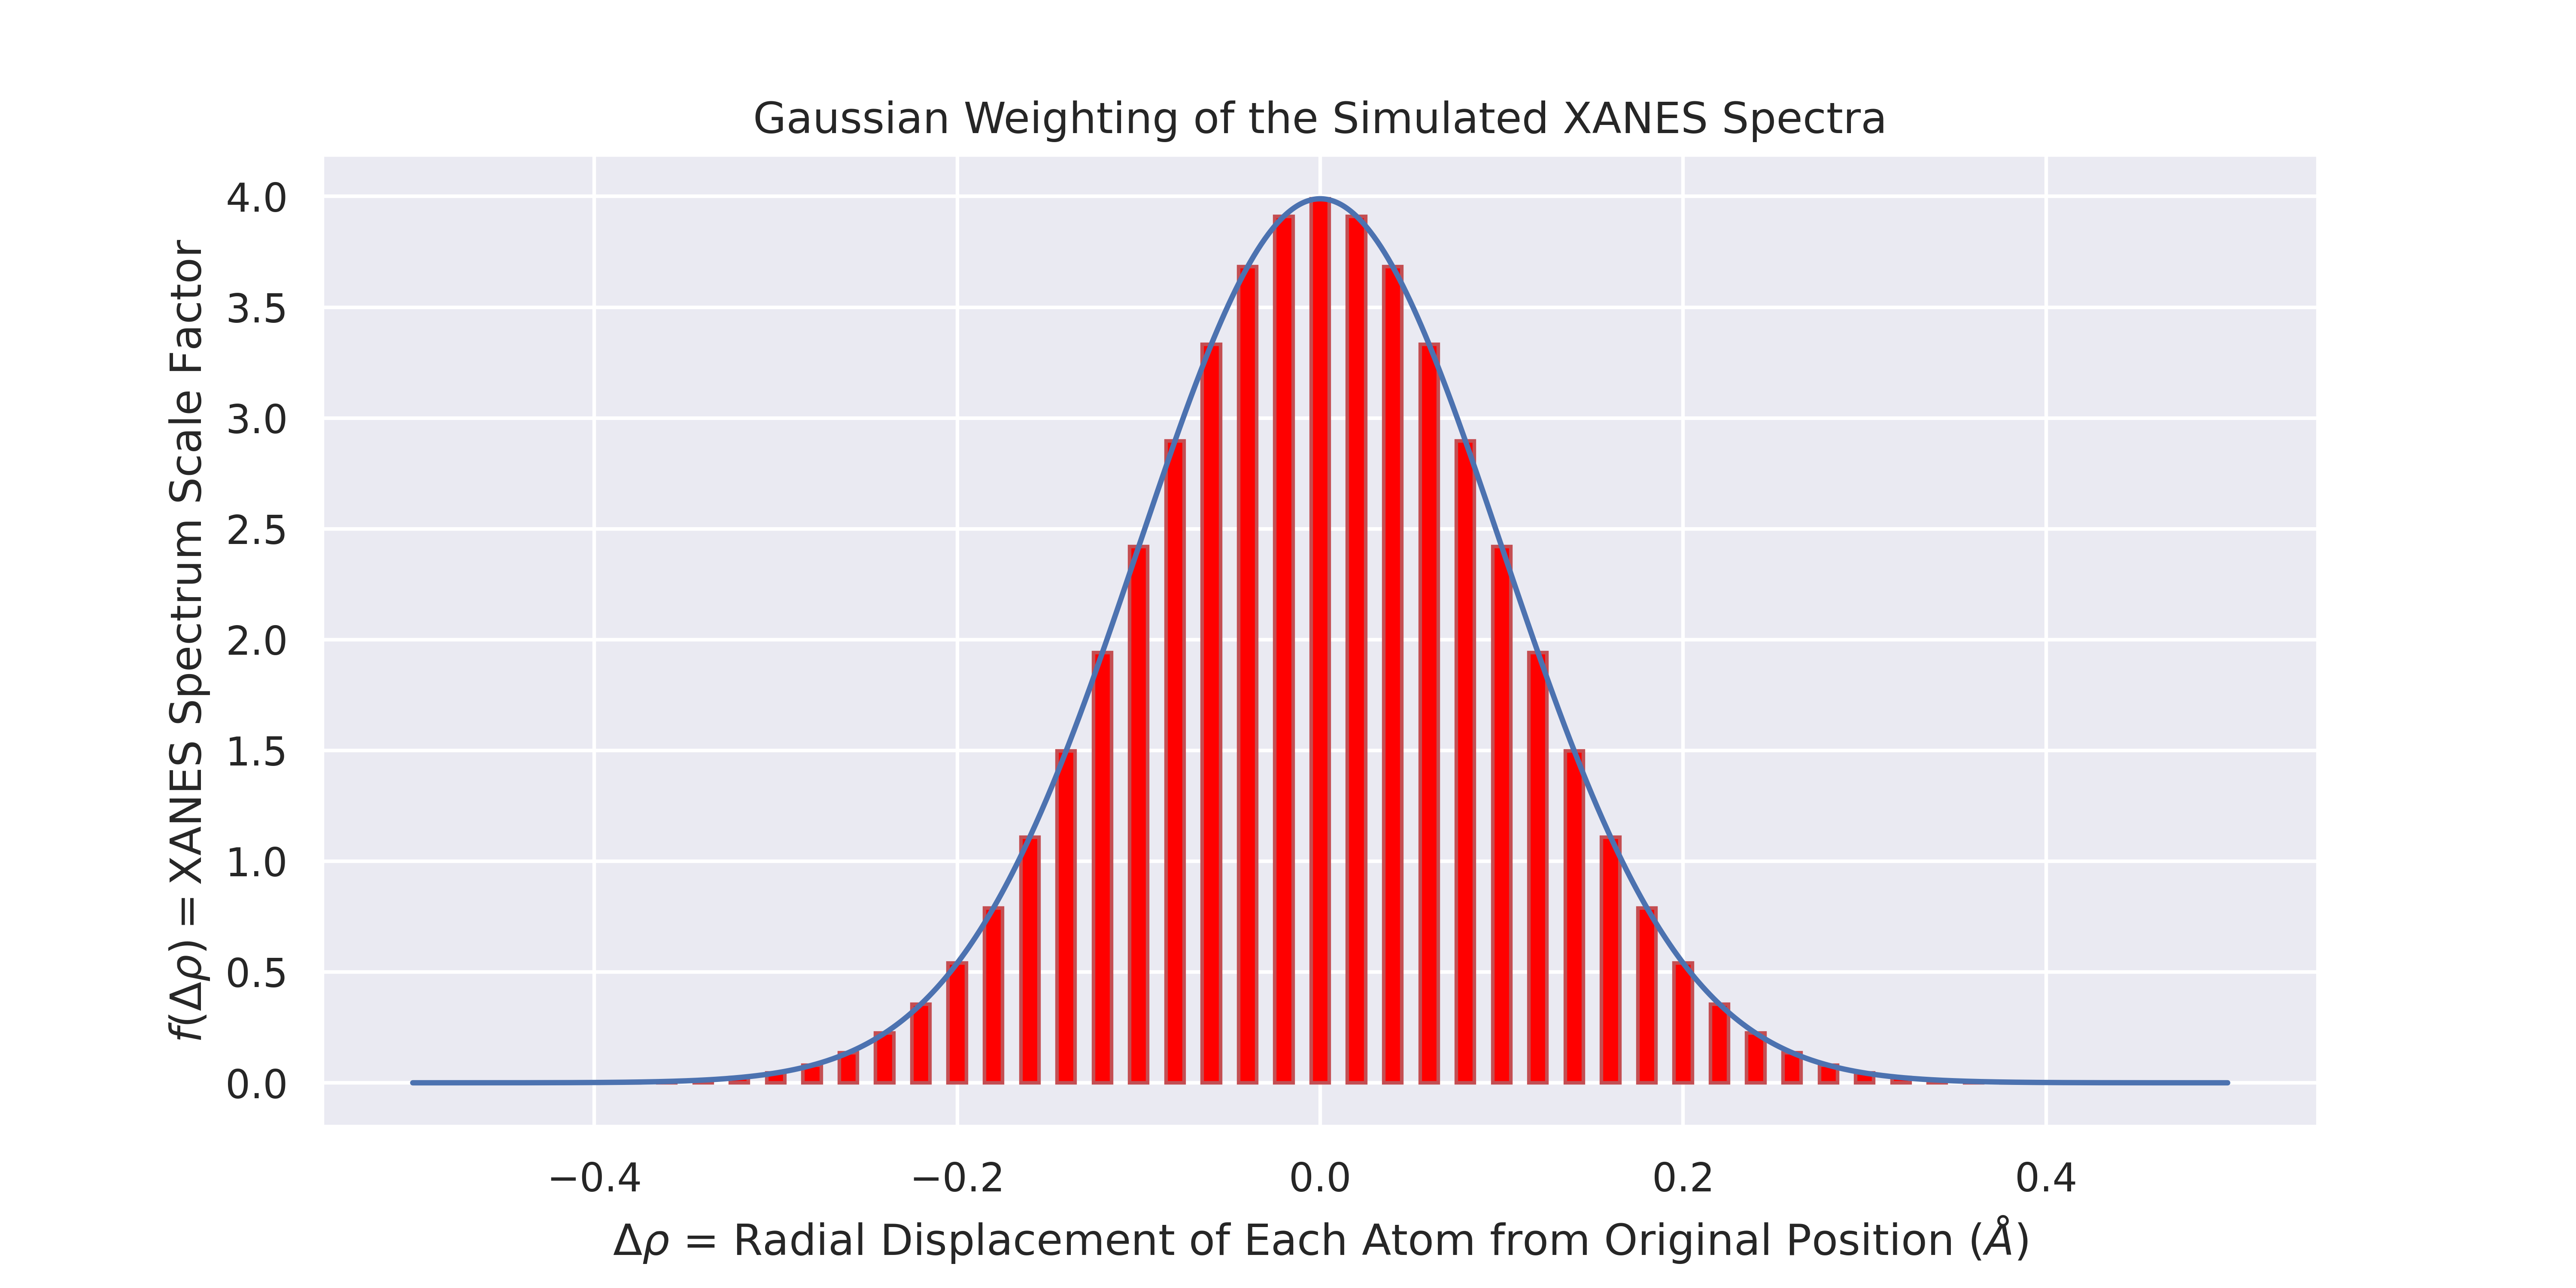
\includegraphics[width=\linewidth]{Chapters/Figures/gaussian-weighting-hist.png}
	\caption[Simulated Spectrum Gaussian Weighting]{A Gaussian distribution probability density function can be used to calculate the relative weight of each FEFF generated XANES spectrum towards one simulated, disordered spectrum. Each bin (red bar) represents a FEFF generated spectrum; the $x$-axis is the isotropic shift of the atomic positions, and the $y$-axis is the relative weight factor.}
	\label{fig:gaussian-weighting-hist}
\end{figure}

The disordered, gaussian-averaged XANES spectrum, $ \left\langle \mu(E) \right\rangle $, using the histogram weighting of the gaussian in Figure \ref{fig:gaussian-weighting-hist} is calculate via Equation (\ref{eqn:gaussian-averaging}):

\begin{equation}
	\label{eqn:gaussian-averaging}
	\left\langle \mu(E) \right\rangle  = \frac{1}{S} \sum_{\Delta\rho=-.45}^{+.45} g\left(\Delta \rho \mid \mu=0, \sigma=0.1\right) \mu(E \mid \Delta\rho)
\end{equation}

\noindent
In the above equation, $ \Delta\rho $ is the isotropic, radial displacement of each atom from its original position, and $ \mu(E \mid \Delta\rho) $ is the simulated FEFF spectrum for the given $ \Delta\rho $ configuration. Furthermore, in Equation (\ref{eqn:gaussian-averaging}), $ S $ represents a standardization factor needed to negate the effect of the changing Gaussian height as a function of the variance, $ \sigma^2 $. With the inclusion of $ S $ , only the relative heights of each bin matters for producing the averaged XANES spectrum. This standardization factor is defined in Eqation (\ref{eqn:gaussian-standardization}):

\begin{equation}
	\label{eqn:gaussian-standardization}
	S = \sum_{\Delta\rho=-.45}^{+.45} g\left(\Delta \rho \mid \mu=0, \sigma=0.01\right)
\end{equation}

\noindent
In both equations (\ref{eqn:gaussian-averaging}) and (\ref{eqn:gaussian-standardization}), the function $ g $ is just the typical Gaussian distribution probability density function (Equation \ref{eqn:gaussian}): 

\begin{equation}
	\label{eqn:gaussian}
	g(x) = \frac{1}{{\sigma \sqrt {2\pi } }}e^{{{ - \left( {x - \mu } \right)^2 } \mathord{\left/ {\vphantom {{ - \left( {x - \mu } \right)^2 } {2\sigma ^2 }}} \right. \kern-\nulldelimiterspace} {2\sigma ^2 }}}
\end{equation}

The above example only generates one (simulated) disordered XANES spectrum and does so via weighting of a Gaussian distribution with mean and variance equal to $ 0 $ and $ 0.01 $, respectively. To simulate systems with different degrees of disorder, we can vary the shape of the probability density function. With a Gaussian distribution, we can only vary the mean and variance; to simulate even more conditions, however, we can instead use the multivariate skew-normal distribution (\ref{eqn:skew-norm}) \cite{skewnorm_Azzalini_1999, 2020SciPy-NMeth}, \textit{f(x)}.

\begin{equation}
	\label{eqn:skew-norm}
	f(x)=2\phi (x)\Phi (\alpha x)
\end{equation}
 
\noindent
where $ \phi(x) $ is the Gaussian PDF:
\begin{equation}
	\label{eqn:skew-norm-pdf}
	\phi (x)={\frac  {1}{{\sqrt  {2\pi }}}}e^{{-{\frac  {x^{2}}{2}}}}
\end{equation}

\noindent
and $ \Phi (x) $ is the Gaussian CDF:
\begin{equation}
	\label{eqn:skew-norm-cdf}
	\Phi (x)=\int _{{-\infty }}^{{x}}\phi (t)\ dt
\end{equation}

%------------WIKIPEDIA EQUATION VERSION -------------
% \begin{equation}
% 	\label{eqn:skew-norm-cdf}
% 	\Phi (x)=\int _{{-\infty }}^{{x}}\phi (t)\ dt={\frac  {1}{2}}\left[1+\operatorname {erf}\left({\frac  {x}{{\sqrt  {2}}}}\right)\right]
% \end{equation}
% \noindent
% and erf is Gauss' error-function

% \begin{equation}
% 	\label{eqn:skew-norm-cdf-erf}
% 	{\displaystyle \operatorname {erf} \left(z\right)={\frac {2}{\sqrt {\pi }}}\int _{0}^{z}e^{-t^{2}}\,dt}
% \end{equation}

\noindent
Equation (\ref{eqn:skew-norm}) includes the shape parameter, $ \alpha $, which has the nice property of producing a right-skewed distribution when positive and a left-skewed distibution when negative. When $ \alpha=0 $, the distribution simply produces the typical Gaussian distribution (eq. \ref{eqn:gaussian}). Utilizing equation (\ref{eqn:skew-norm}), we can vary $ \mu, \sigma,  $ and $ \alpha $ to alter the first four moments of the function: mean, standard deviation, skew, and kurtosis. Eighteen possible skew-norm weighting functions are plotted in Figure \ref{fig:skew-norm-options}. To produce the neural network training data, 1000 such weightings are used.

\begin{figure}[h!]
	\centering
	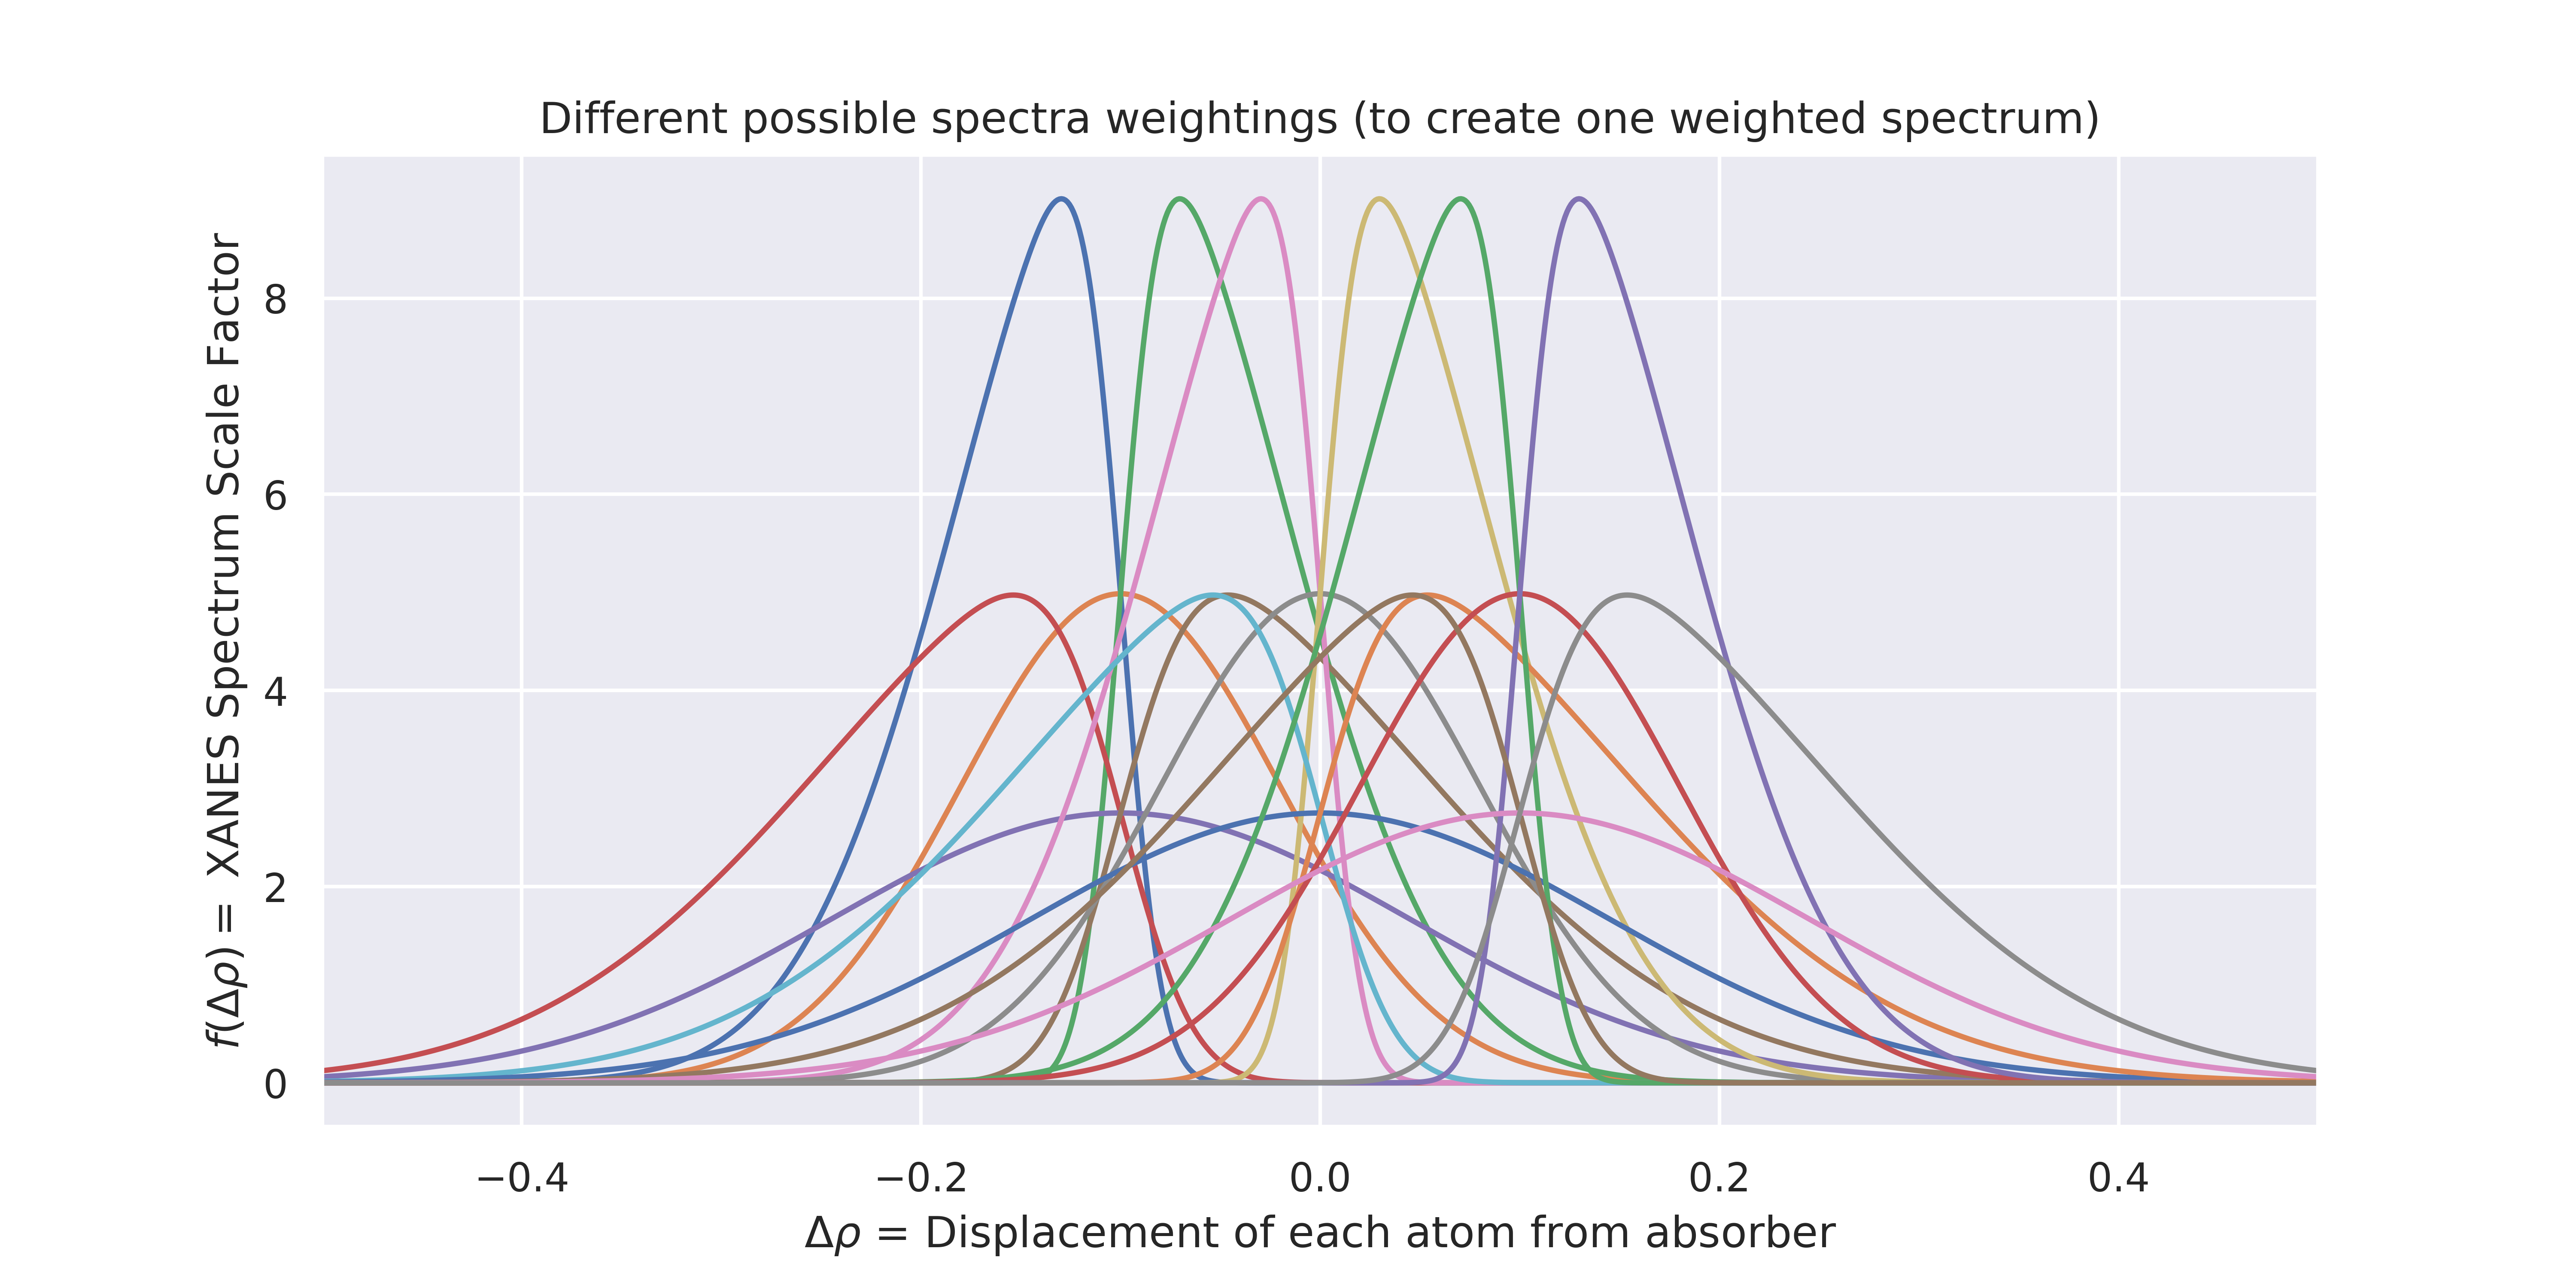
\includegraphics[width=\linewidth]{Chapters/Figures/skewnorm_options.png}
	\caption[Simulated Disordered Spectrum Weightings]{Eighteen skew-norm distributions plotted with all possible combinations of $ \sigma=\{.08, .145\} $, $ \mu=\{-.1, 0, .1\} $, and $ \alpha=\{-5,0,5\} $. Each represents a possible way to produce a simulated, disordered spectrum from many FEFF-simulated, distorted spectra} 
	\label{fig:skew-norm-options}
\end{figure}

The disorder of the skew-norm generated, disordered spectrum is characterized by the mean squared displacement of each atom from its original position ($ \Delta\rho $ ), weighted in the same manner as the spectra. \textit{Instead of characterizing the disordered spectrum by the standard deviation of the gaussian used to create it.} The weighted mean squared displacement, $ MSD $, is calculated via equation (\ref{eqn:weighted-MSD}):

\begin{equation}
	\label{eqn:weighted-MSD}
	MSD  = \frac{1}{S} \sum_{\Delta\rho=-.45}^{+.45} f\left(\Delta \rho \mid \mu, \sigma^2, \alpha \right) 
\end{equation}

\noindent
Here, $ f(x) $ is the skew-norm function from equation (\ref{eqn:skew-norm}), and the $ MSD $  of each individual FEFF spectrum is equal to the isotropic distortion, $ \Delta\rho $.  

\section{Simulation vs. Experimental Data} \label{sec:end-disorder}

To check our FEFF simulation parameters, as well as the validity of the gaussian-weighted disorder technique, we compare the simulation data to experimental data. \textit{Can someone give me citations for these?} In Figure \ref{fig:avg-experimental-vs-simulation}, both experimental and simulation spectra for bulk-like and nanoparticle scenarios are plotted. EXAFS fitting was used to characterize the disorder in the experimental measurements. For the bulk foil, this parameter was found to be $ \sigma^2=0.0081(5)~$ {\AA}$ ^2 $, and for the 8~nm disordered particle, $ \sigma^2=0.0102(8) $~{\AA}$ ^2 $.  One simulated, disordered spectrum was weighted according to the gaussian $ N(0, 0.09) $ to represent the disordered nanoparticle, and the other was weighted according to the gaussian $ N(0, 0.038)  $ to represent the bulk. These weightings correspond to $ MSD $ values that match the measured $ \sigma^2 $ values for the experimental data.  

\begin{figure}[h]
	\centering
	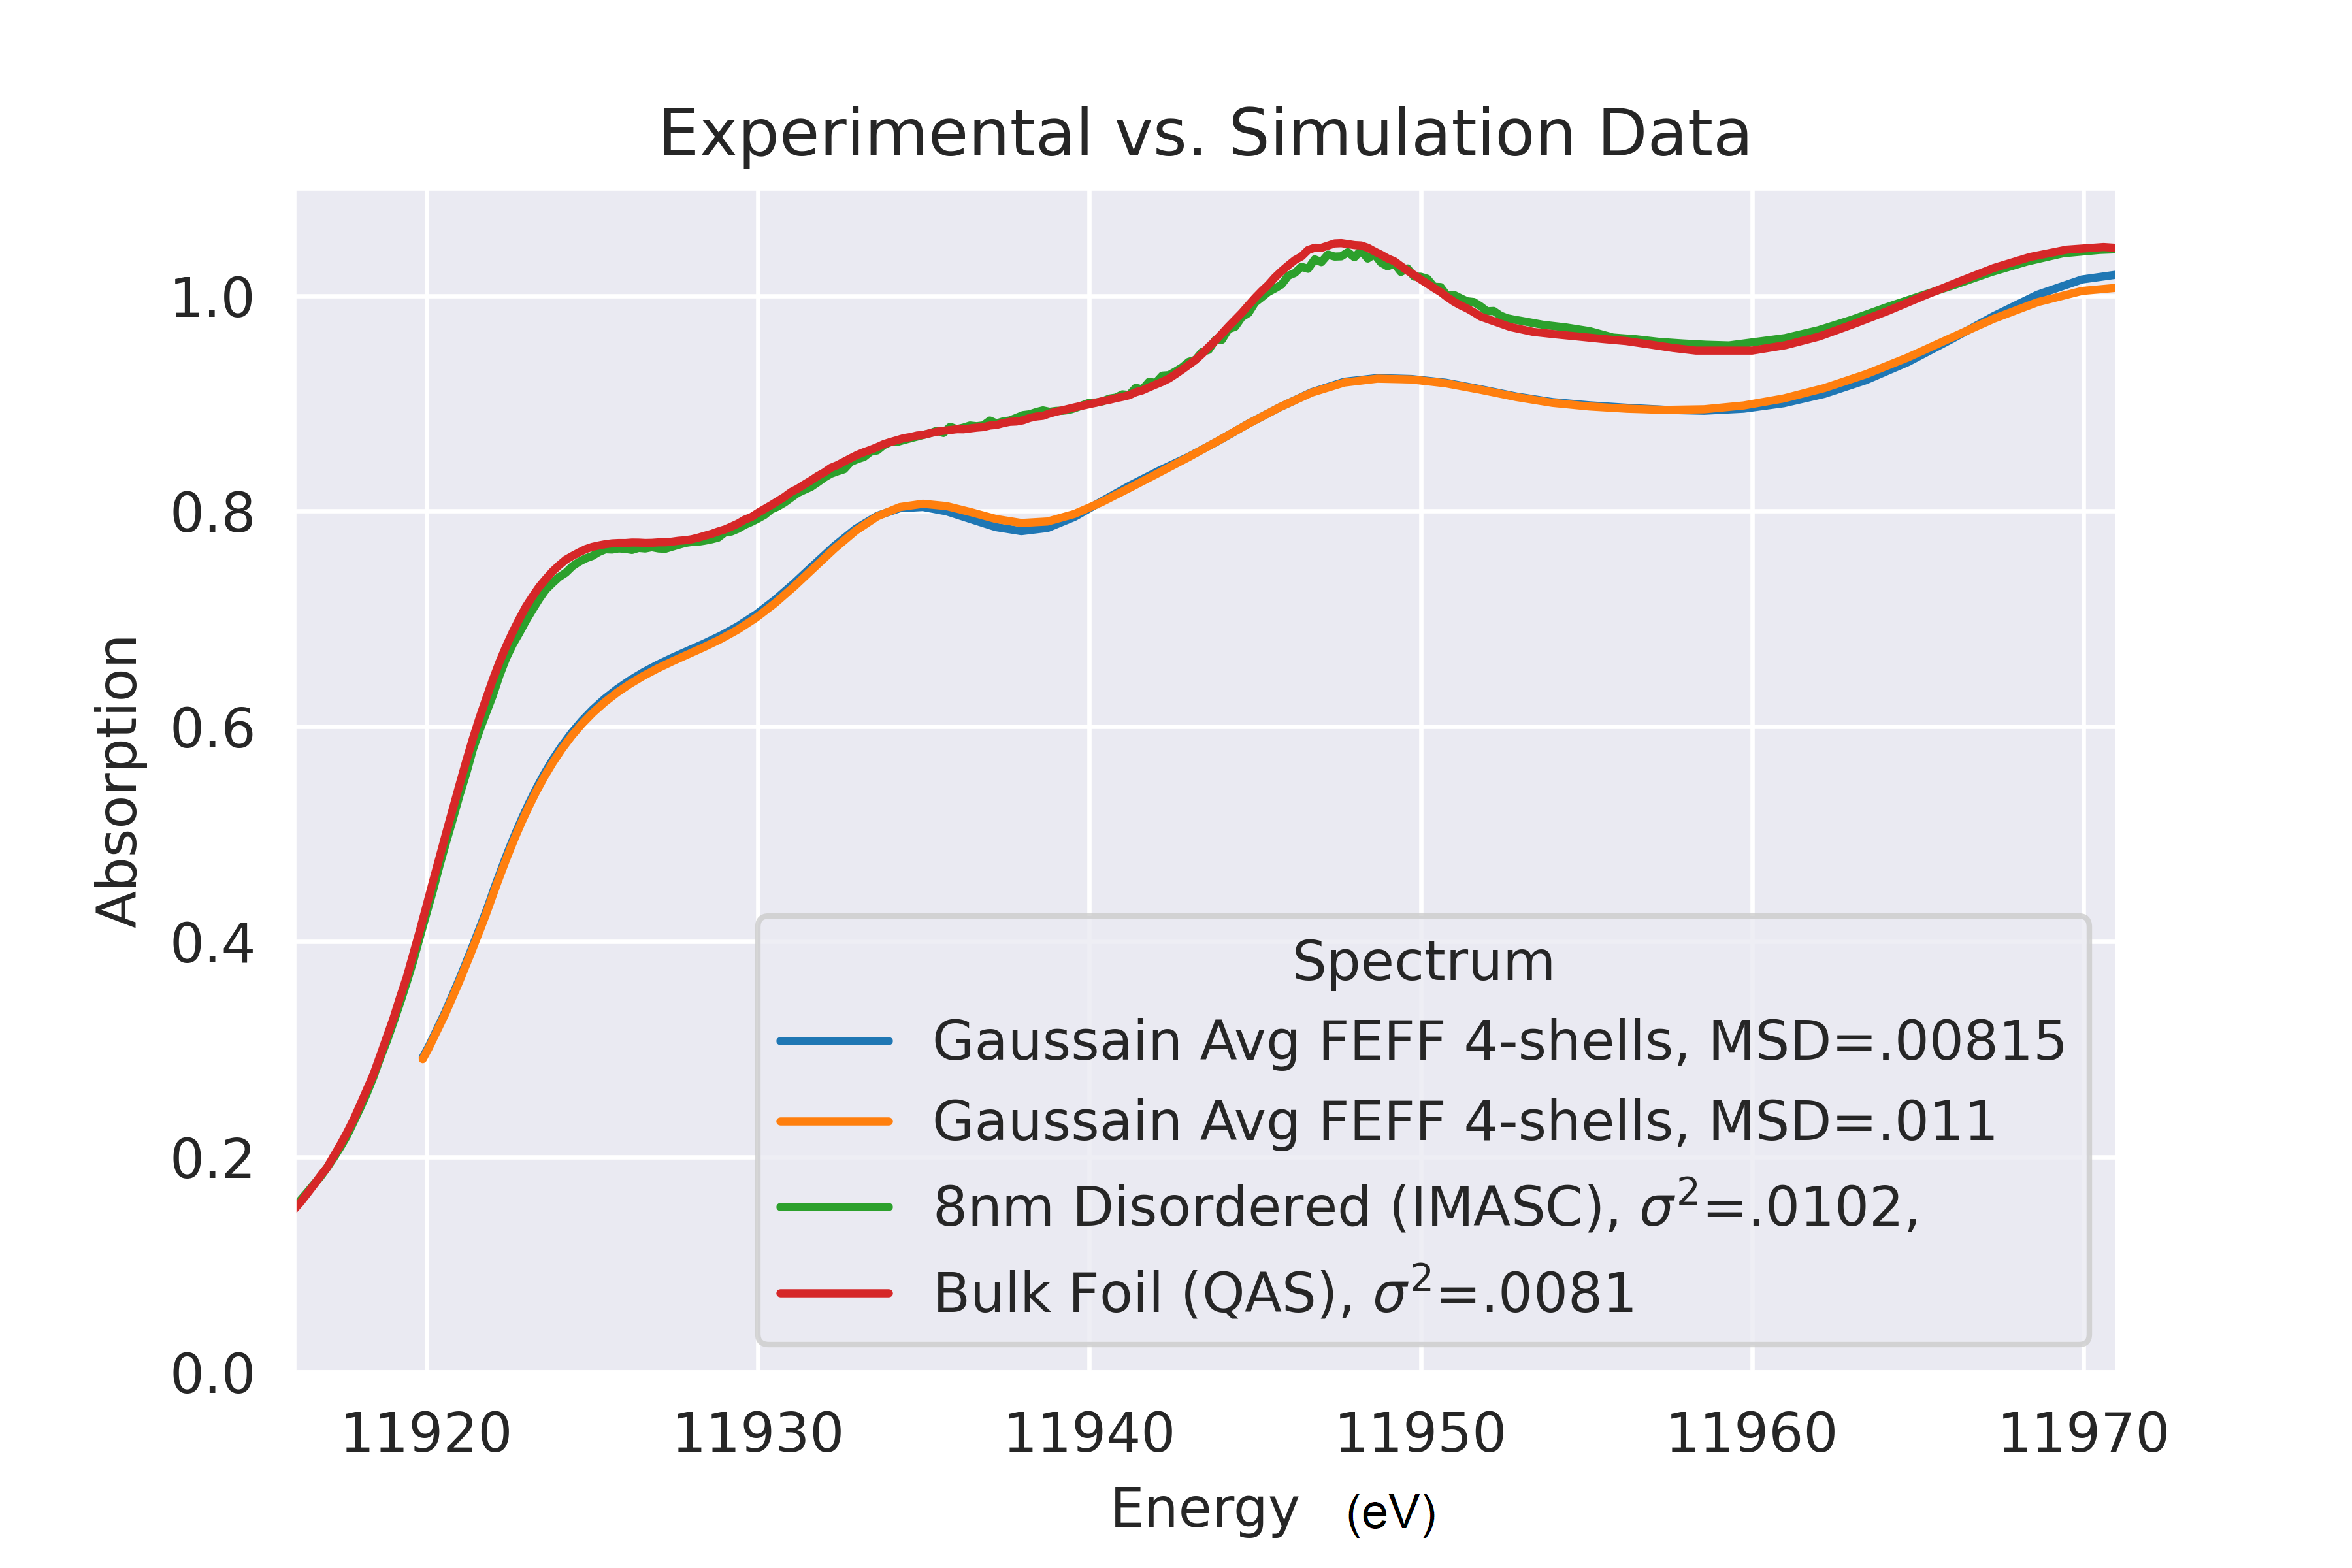
\includegraphics[width=.75\linewidth]{Chapters/Figures/updated_bulk_8nm_disorder_experimental_theory_comparison.png}
	\caption[Simulation vs. Experimental]{Comparing the bulk foil (red) measurement to the 8~nm disordered nanoparticle (green) measurement is an analog to comparing the simulated, non disordered FEFF spectrum (blue) to the simulated disordered spectrum (orange).}
	\label{fig:avg-experimental-vs-simulation}
\end{figure}

In Figure \ref{fig:avg-experimental-vs-simulation}, the bulk Au foil spectrum is above the 8~nm nanoparticle spectrum (more absorption) until the peak around 11937~eV, where the NP absorption becomes higher. The two criss-cross again over the next two peaks, changing which material has the higher absorbance in an energy range. This change is more easily seen in Figure \ref{fig:avg-experimential-vs-simulation-difference}, which plots the difference between the the bulk material and the nanoparticle absorption for both the experimental measurements and the simulations. The experimental and simulation difference-spectra follow the same trend with the exception of the peak around 11947~eV.
% The two spectrum switch again at the peak around 11943~eV so the bulk foil's absorption nlevel is higher again. Beyond this peak, the two


\begin{figure}[h!]
	\centering
	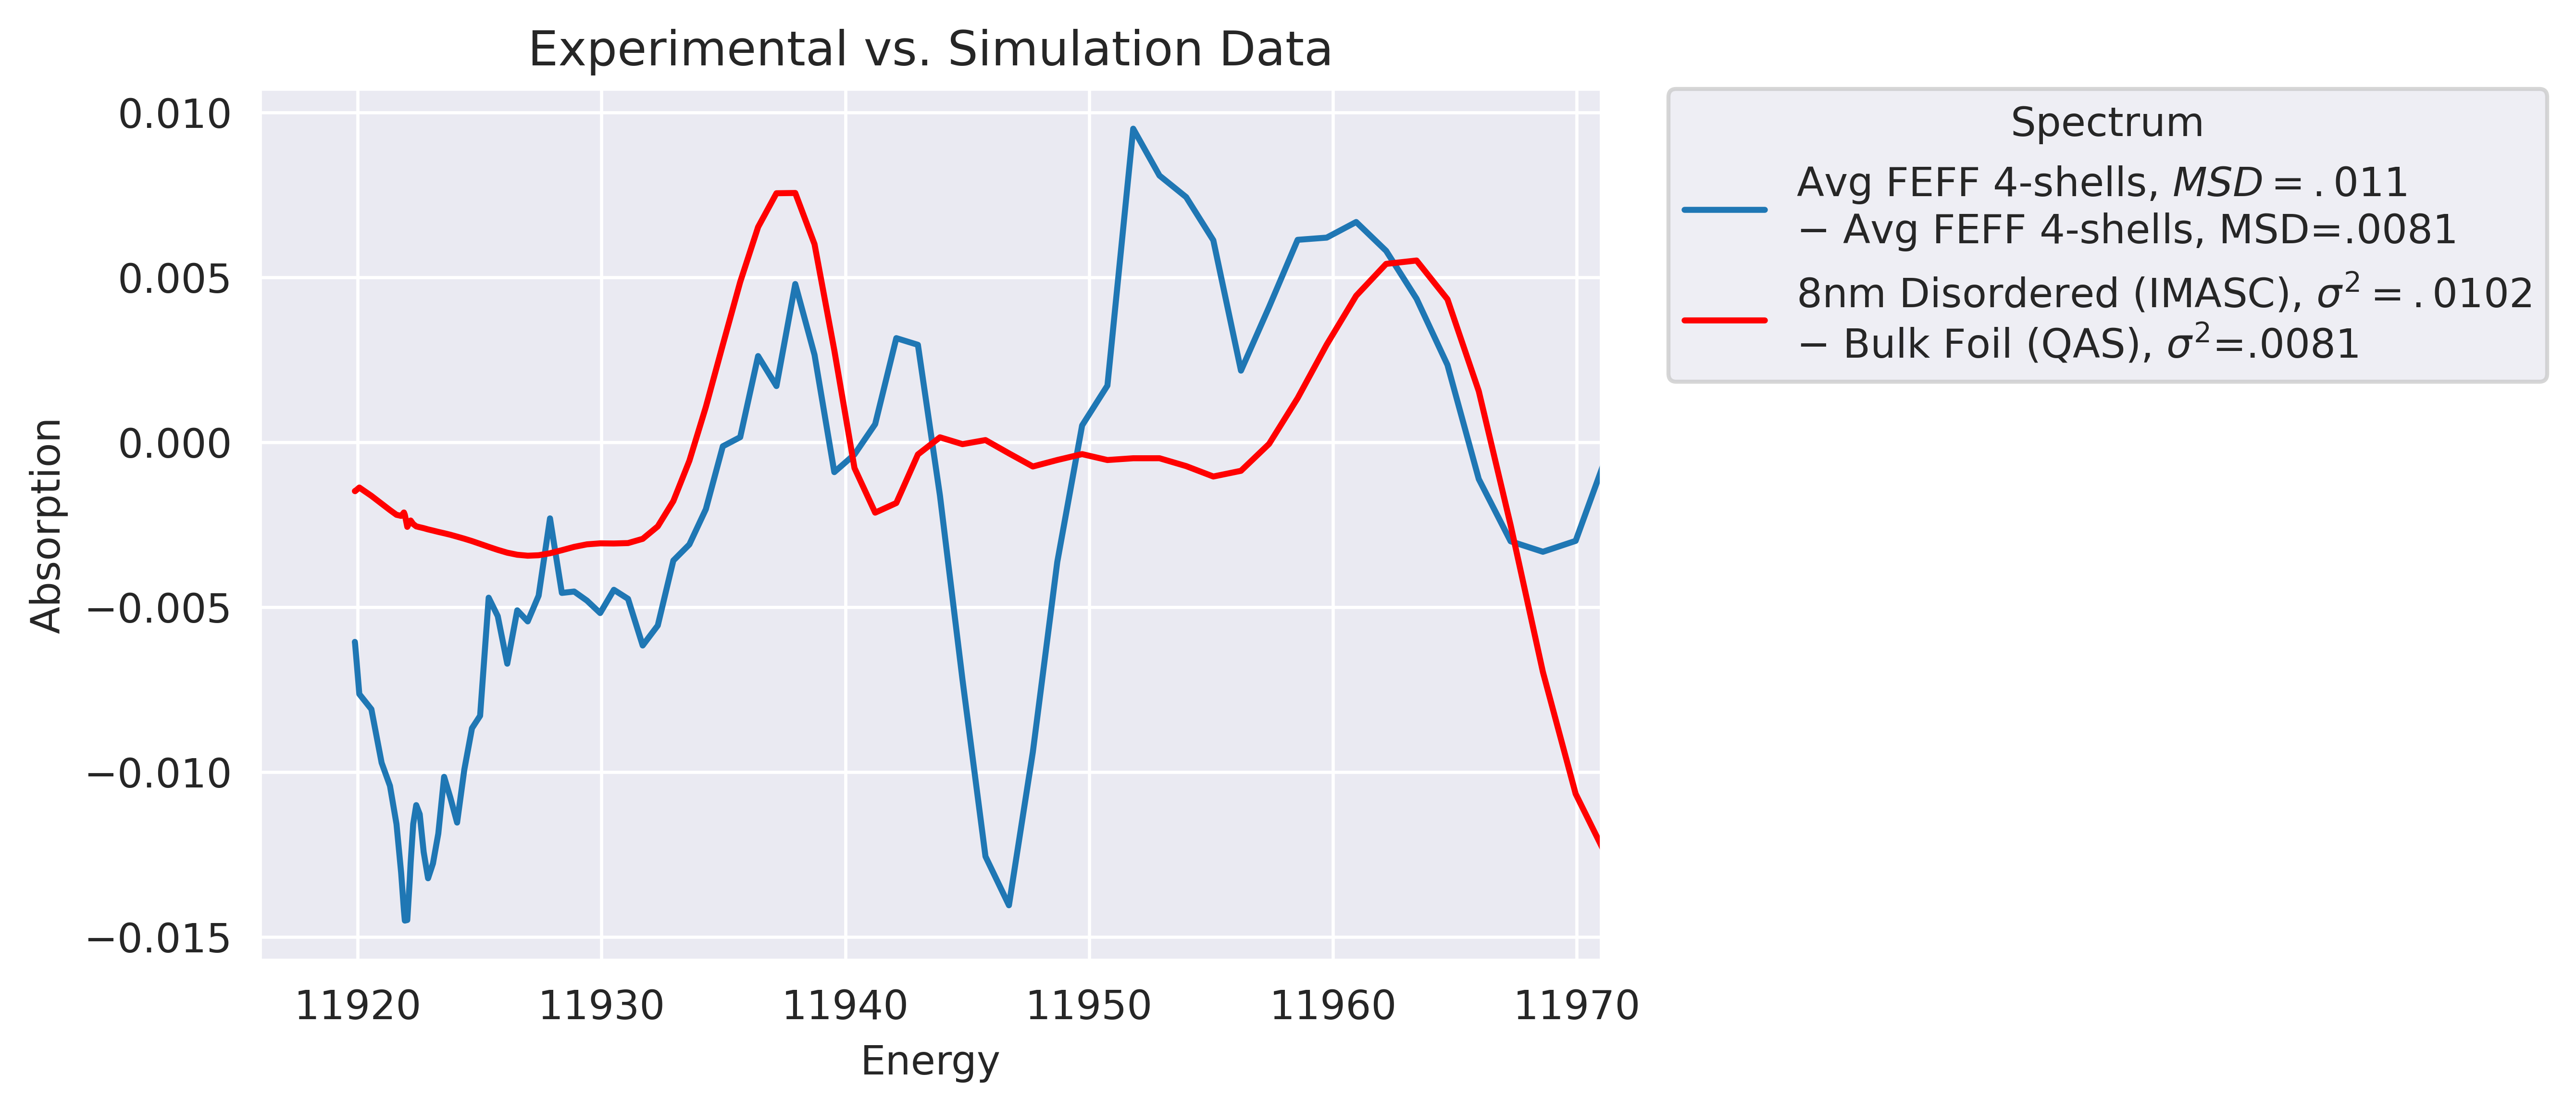
\includegraphics[width=\linewidth]{Chapters/Figures/experimental_vs_simulation_delta.png}
	\caption[Bulk-nanoparticle difference: Simulation vs. Experimental data]{The difference between the nanoparticle spectrum and the bulk spectrum are plotted for the same data as in Figure \ref{fig:avg-experimental-vs-simulation}. It is easier to see where the bulk and the nanoparticle absorption crisscross by plotting the difference.}
	\label{fig:avg-experimential-vs-simulation-difference}
\end{figure}

Figures \ref{fig:avg-experimental-vs-simulation} and \ref{fig:avg-experimential-vs-simulation-difference} aren't meant to be perfect comparisons of simulations vs. experimental data. For one, the experimental data compares a bulk spectrum to a nanoparticle. By contrast, both the simulation spectra are of the same size 55 atom cluster. Still, much of the disorder trends are coded in the simulation approach. 

To test if the size information is also coded in our simulations, we compare different size simulations to experimental data in Figure \ref{fig:avg-experimental-vs-simulation2}. As expected, including more atoms in the simulation produces more bulk-like spectrum characteristics, such as larger amplitude peaks.

\begin{figure}[h]
	\centering
	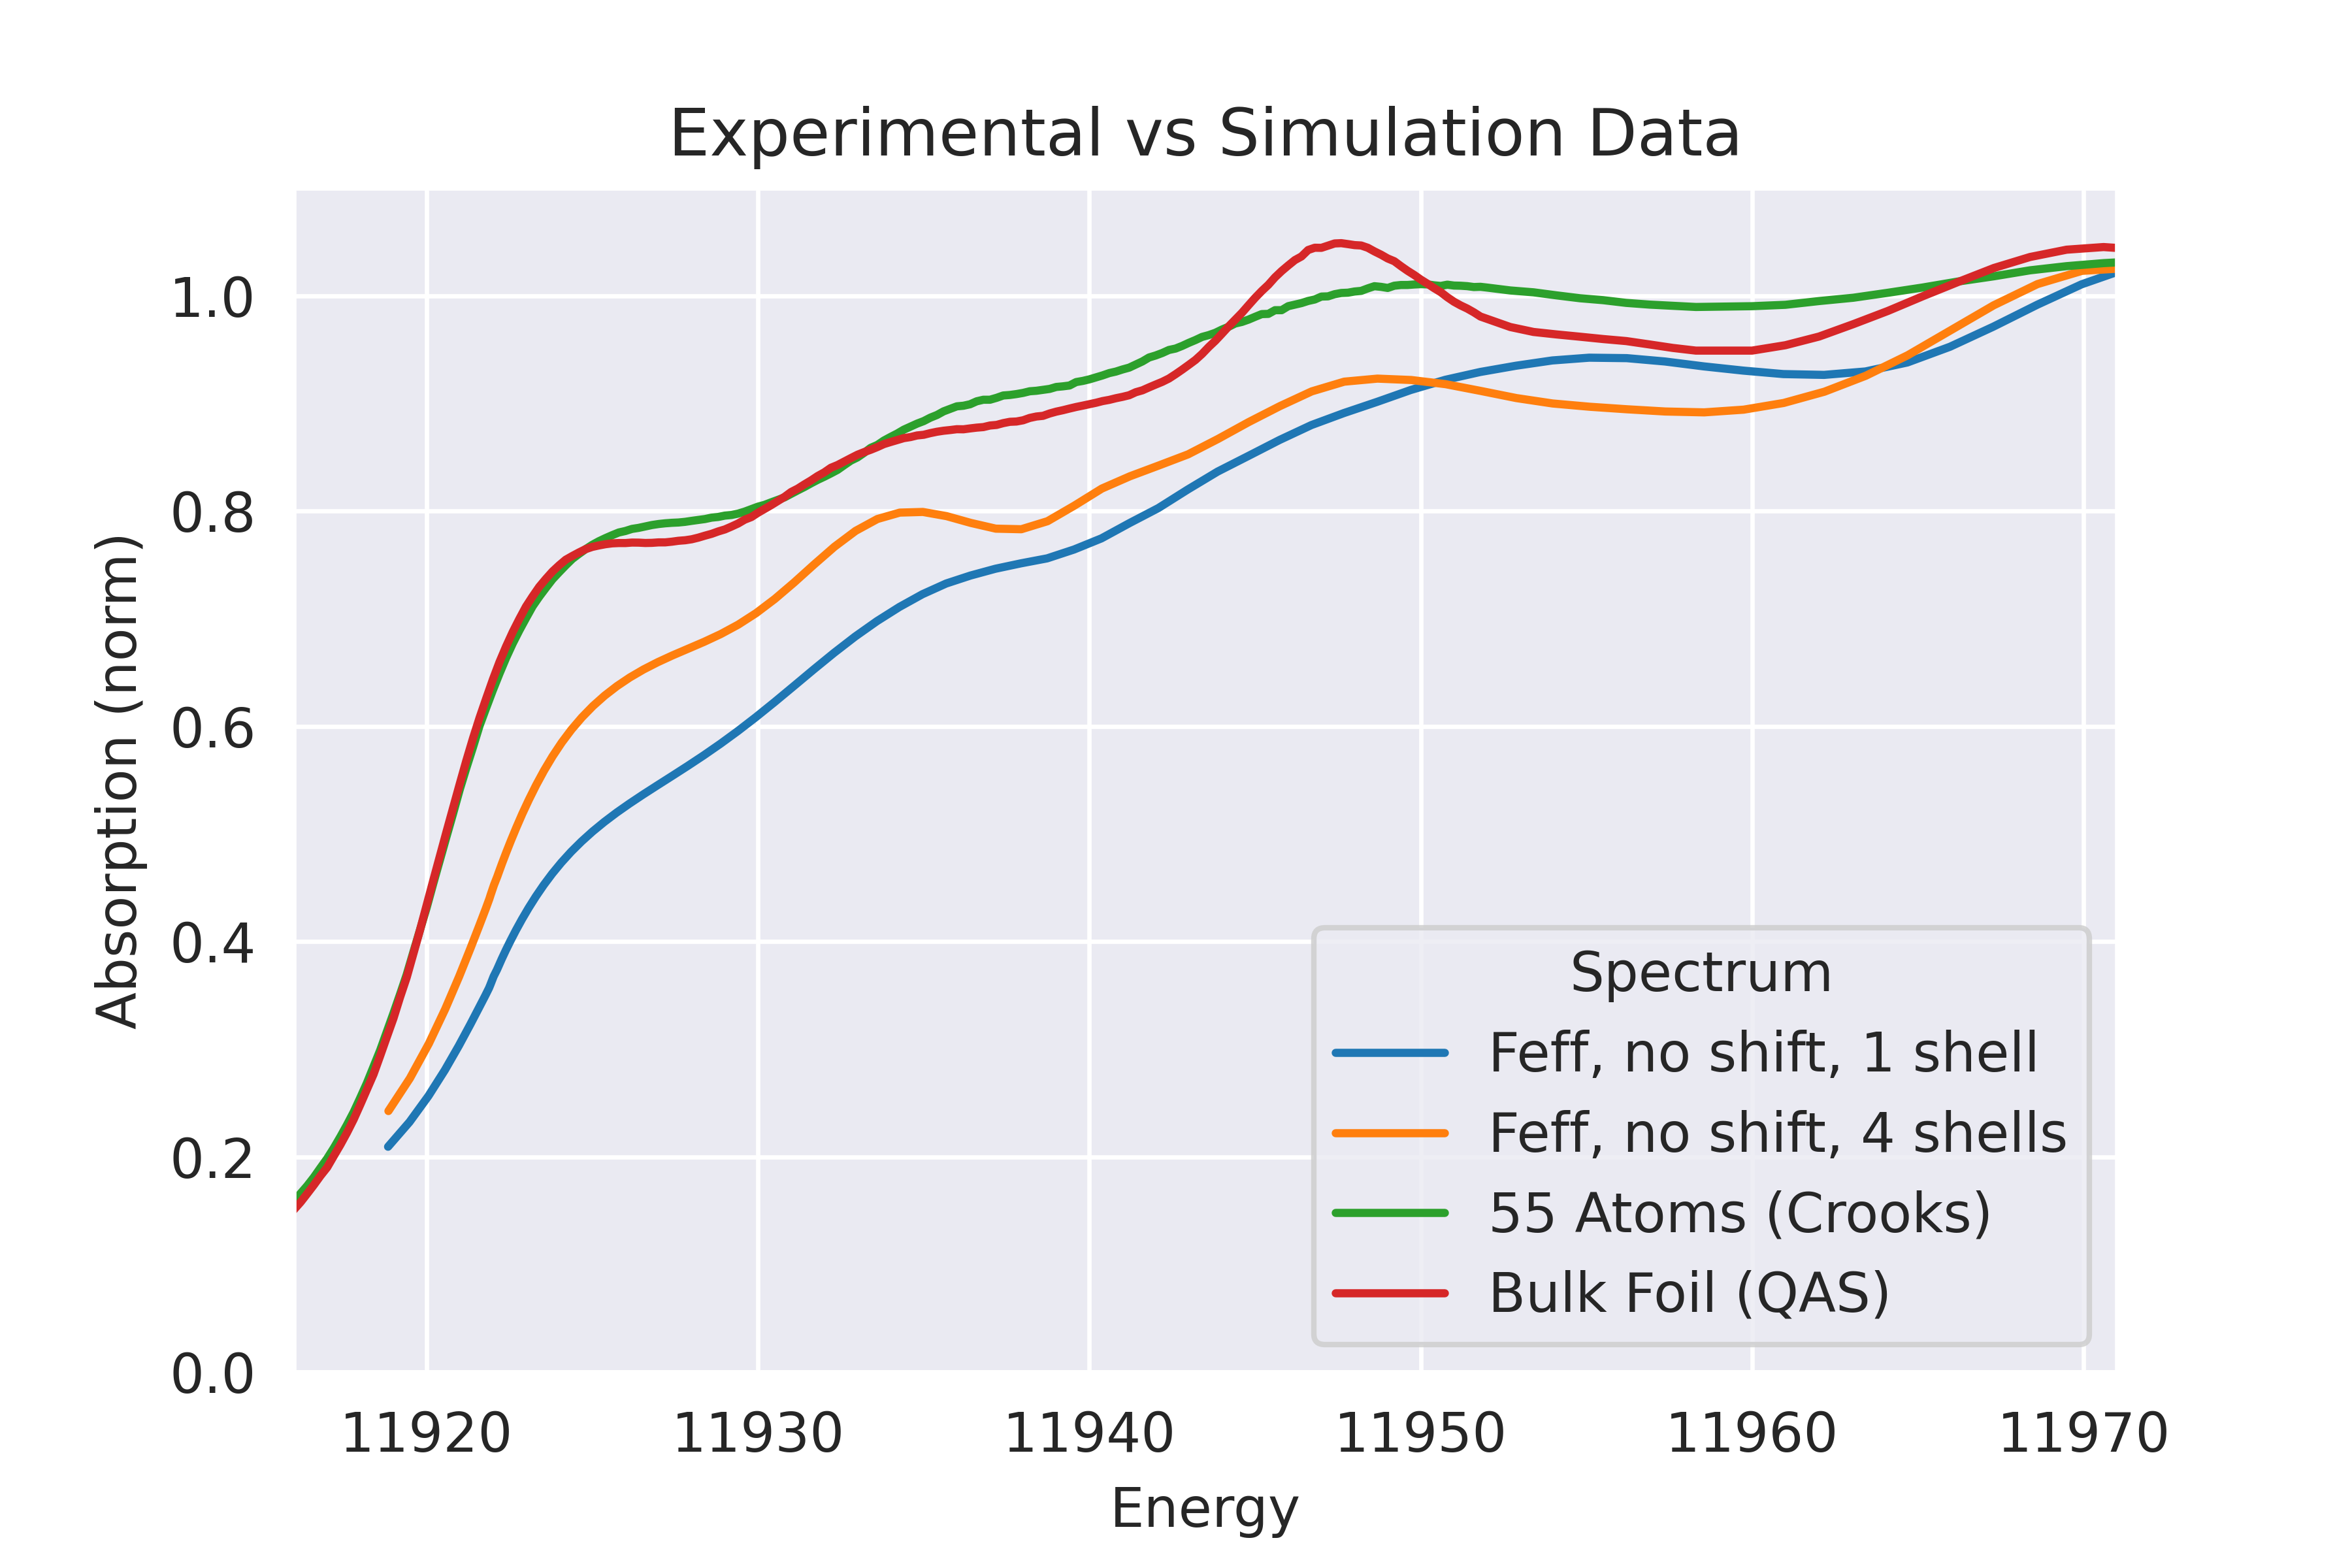
\includegraphics[width=.7\linewidth]{Chapters/Figures/Bulk_55atom_experimental_theory_comparison.png}
	\caption[Simulation vs. Experimental 2]{Comparing the bulk foil (red) measurement to the 55 atom nanoparticle (green) measurement is an analog to comparing the 13 atom simulated spectrum (blue) to the 55 atom simulated spectrum (orange).}
	\label{fig:avg-experimental-vs-simulation2}
\end{figure}

I NEED A PLOT COMPARING THIS METHOD TO PARTICLE AVERAGED METHOD HERE.

\section{Particle-Averaged FEFF Simulated Disordered Structures} \label{sec:pa-feff-vs-gaussian-feff}

\begin{figure}[h]
	\centering
	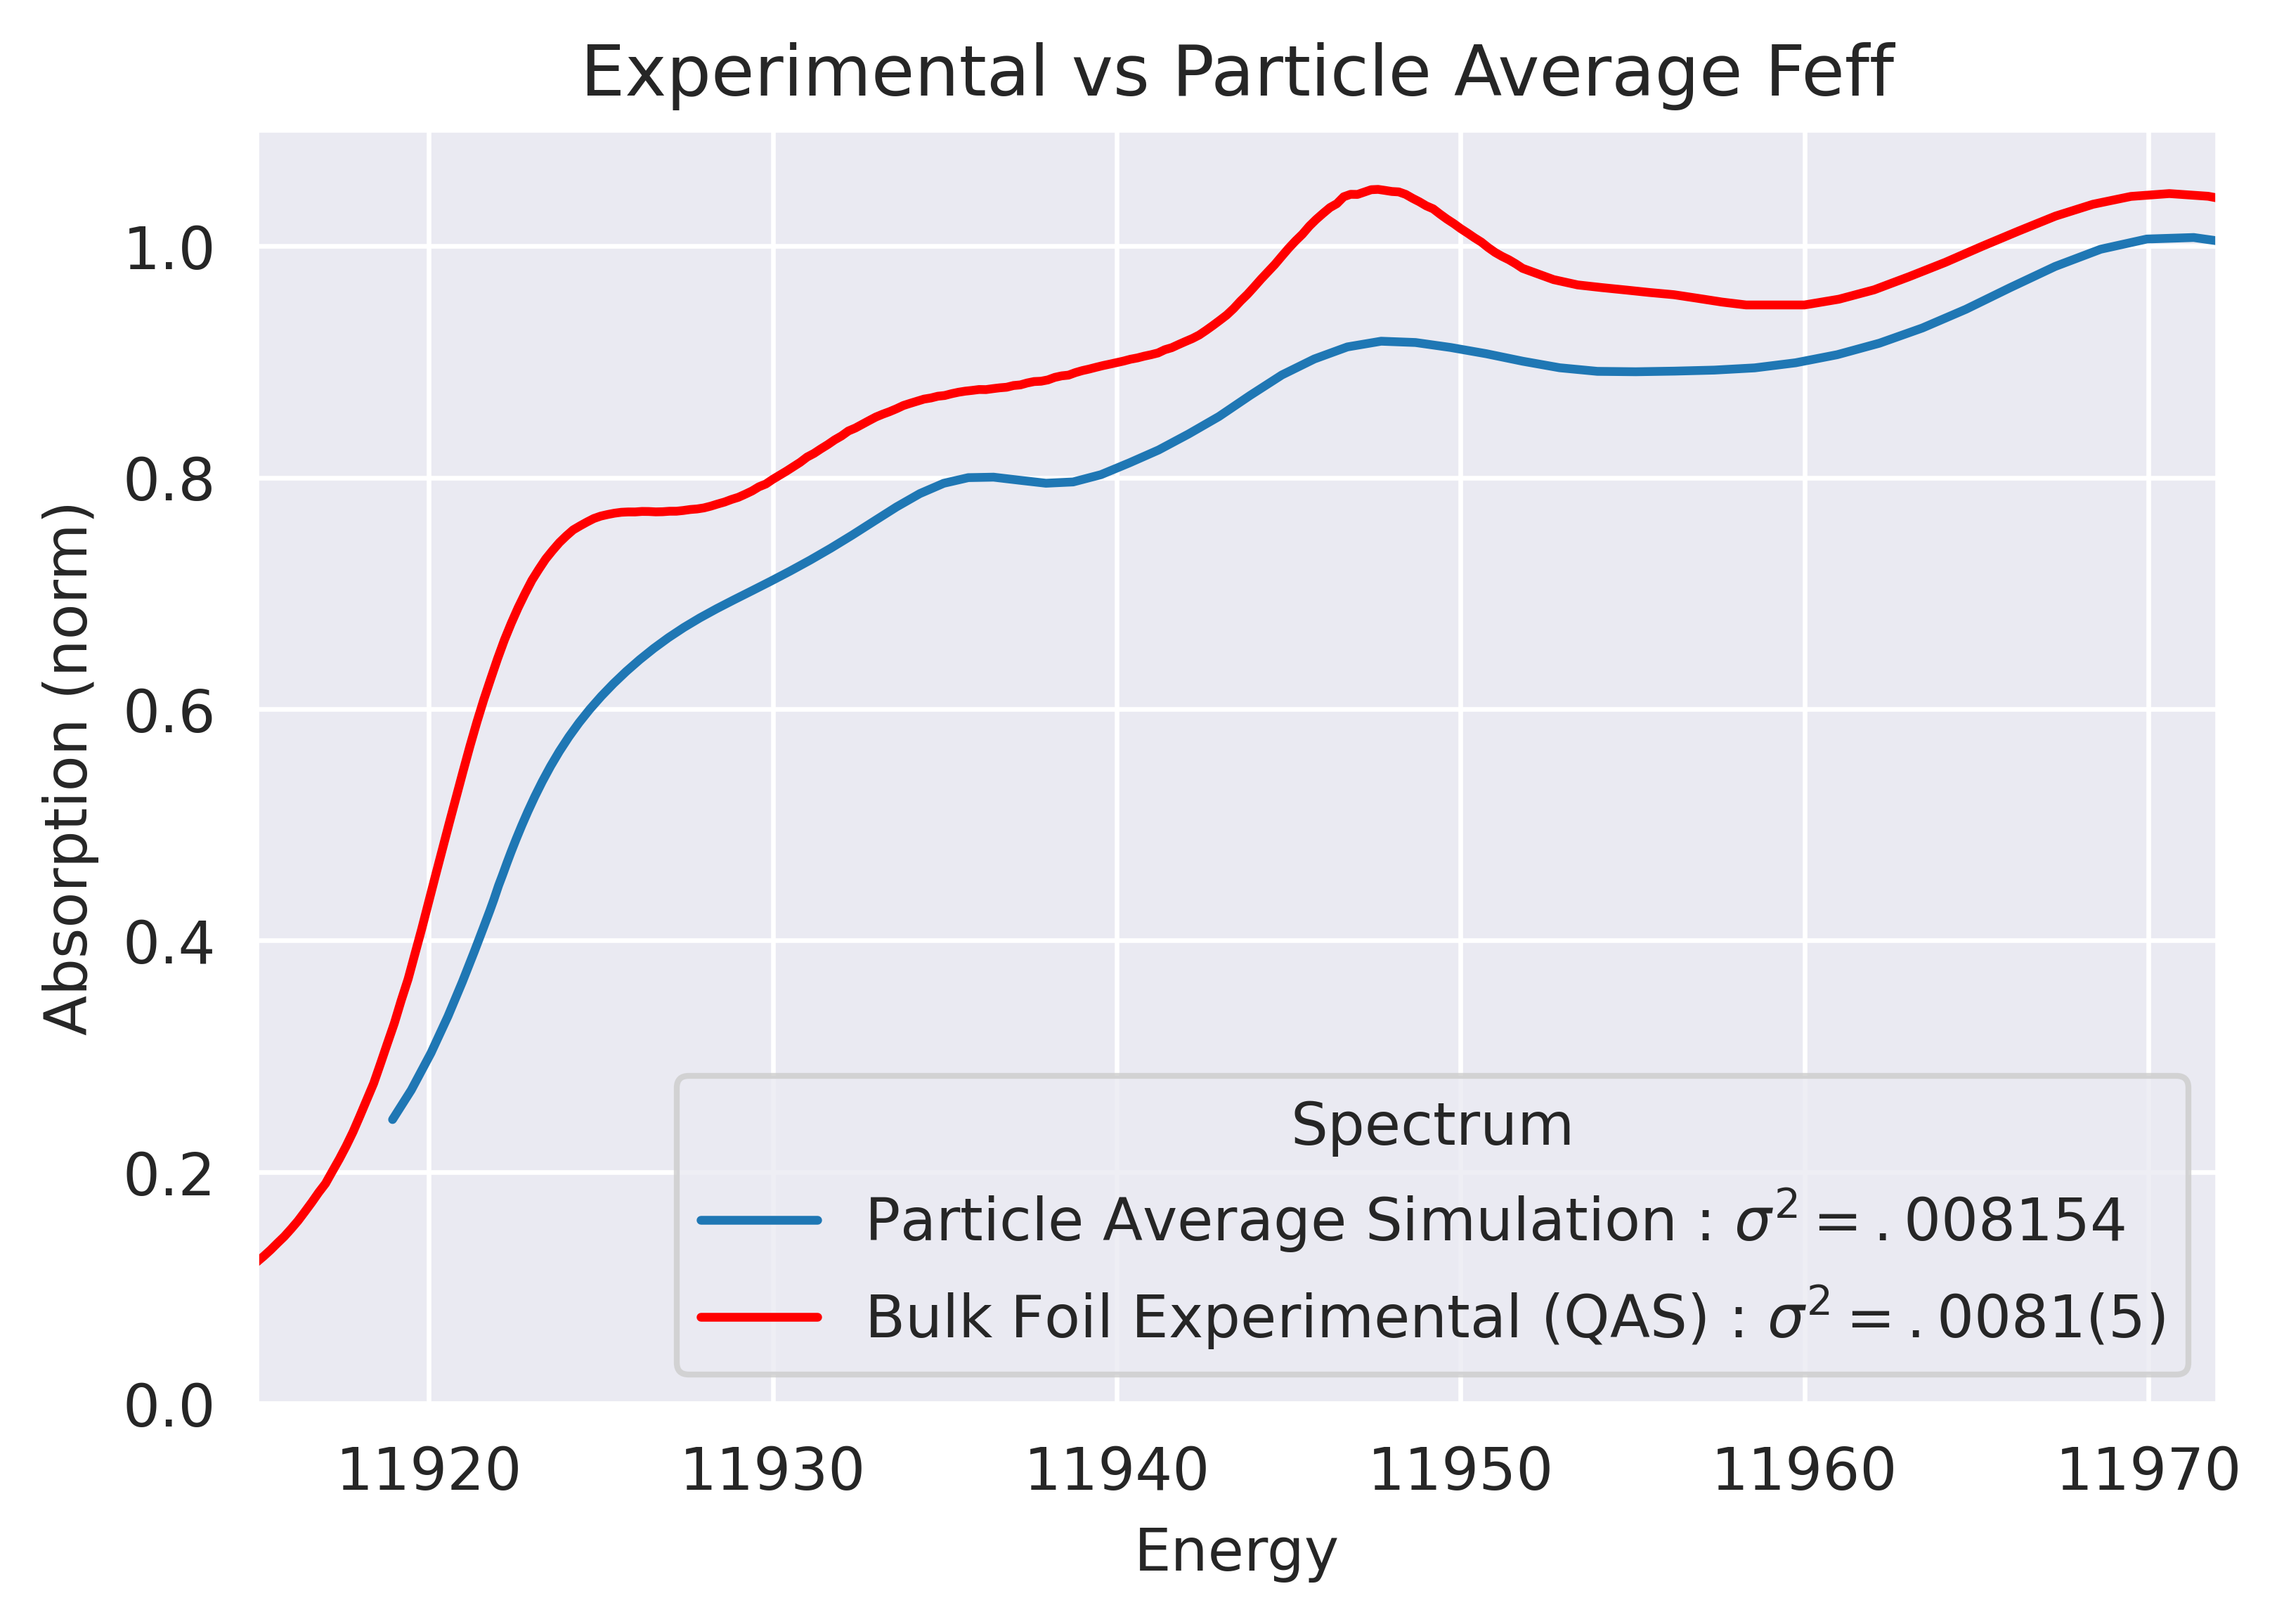
\includegraphics[width=.7\linewidth]{Chapters/Figures/Bulk_experimental_vs_pa_comparison.png}
	\caption[Simulation vs. Experimental 3]{Comparing the bulk foil (red) measurement to a simulated large, bulk-like nanoparticle with the same disorder. The FEFF-}
	\label{fig:avg-experimental-vs-simulation2}
\end{figure}

\section{Traditional Particle-Averaged Simulations} 
\label{sec:traditional-disorder}


% the \appendix tag tells LaTeX where it should start labeling chapters with letters (denoting appendices) rather than numbers (denoting main chapters)
\appendix 


\chapter{An appendix}
% Look!  An Appendix!

% Appendices are a good idea for almost any thesis.  Your main thesis body will likely contain perhaps 40-60 pages of text and figures.  You may well write a larger document than this, but chances are that some of the information contained therein, while important, does \emph{not} merit a place in the main body of the document.  This sort of content - peripheral clarifying details, computer code, information of use to future students but not critical to understanding your work \ldots - should be allocated to one or several appendices.  

\section{distortionator.py}
Given \texttt{feff.inp} file, generate many \texttt{feff.inp} files --- each with a structure slightly shifted radially outwards (or inwards) from the original structure. File structure is organized as the following: 

\begin{minipage}{\linewidth}
~ \\
\begin{Verbatim}[samepage=true]
    BNL
    │   distortionator.py
    │   gaussianator.py
    │       
    └───DATA
    │   │       
    │   │
    │   └───Original_Structure
    │   │   │   feff.inp
    │   │       
    │   └───minus_pt_0001
    │   │   │   feff.inp
    │   │       
    │   └───plus_pt_0001
    │   │   │   feff.inp
    │   │
    │   ....        
\end{Verbatim}
~
\end{minipage}

\section{gaussianator.py} \label{appendix:gaussianator}
Take all the \texttt{xmu.dat} files (each one represents the sprectrum from the $\Delta \rho$ shifted crystrals) and generates many gaussian averaged XANES spectra. One file per different standard deviation of the gaussian. The File structure is organized as follows: 

\begin{minipage}{\linewidth}
~ \\
\begin{Verbatim}[samepage=true]
    BNL
    │   distortionator.py
    │   gaussianator.py   
    │
    └───DATA
    │   │ 
    │   └───Averaged_Spectra
    │       │       
    │       │   sigma_0001.csv
    │       │   sigma_0002.csv
    │       │   ...      
\end{Verbatim}
~
\end{minipage}

\begin{lstlisting}[language=Python]
    # Inputs: -----
    # dataframe df = the already mapped concat dataframe of all the different delta_rho shifted feff xanes
    # float64 mean = mean of gaussian.
    # float64 std = standard deviation of gaussian
    # float64 skewness = skew parameter of stats.skewnorm
    # Outputs: ----
    # dataframe df_weighted2 = one dataframe. It is one distribution-weighted spectra with cols=['omega','mu']
    # float64 avg_MSD = the mean squared displacement of the skewnorm-averaged spectrum
    # Note a skewness of 0, sigma 1, and mean 0 is a standardized normal distribution.
    def weight_by_distribution2(df_concat, mean, std, skewness):
    # ---------
    # get the bin heights for all the bins
    bin_heights = np.array([stats.skewnorm.pdf(nn_dist, loc=mean, scale=std, a=skewness) for nn_dist in BINS])
    normalization_factor = np.sum(bin_heights)
    # same as sum(bin_height_i * nn_bond_dist)/(sum(bin_heights))
    weighted_nn_dist_mean = np.dot(bin_heights, BINS) / normalization_factor
    # same as sum(bin_height_i * ( nn_bond_dist_i - mean_bond_dist )^2 )/sum(bin_heights)
    sq_dif = np.square(np.subtract(BINS, weighted_nn_dist_mean))
    avg_msd = np.divide(np.dot(bin_heights, sq_dif), normalization_factor)
    # now do the spectrum -----------------
    df_weighted2 = pd.DataFrame(data={'omega': df_concat.loc['0'].omega, 'mu': np.zeros(df_concat.loc['0'].omega.shape[0])})
    for shift, bin_height in zip(SHIFTS, bin_heights):
        df_weighted2.mu += df_concat.loc[shift]['mu'].multiply(bin_height)
    df_weighted2.mu /= normalization_factor  # correct for the sum, so the area under the PDF=1
    return df_weighted2, avg_msd
\end{lstlisting}
    

\section{generate-training-data.py}
This script generates the FEFF input files (\texttt{feff.inp}) for the disordered structures---i.e. the true-disordered structures, NOT the distorted structures used for the skew-norm averaging.

\begin{minipage}{\linewidth}
    ~ \\
    \begin{Verbatim}[samepage=false]
        BNL
        │   distortionator.py
        │   gaussianator.py
        │   generate-training-data.py
        │       
        └───DATA
        │   │       
        │   │
        │   └───MSD-0
        │   │   │   avg_msd.txt
        │   │   │
        │   │   └── 0
        │   │   │   │   feff.inp
        │   │   │   │   msd.txt
        │   │   ...
        │   │   │
        │   │   └── 12
        │   │       │   feff.inp
        │   │       │   msd.txt
        │   │       
        │   ...
        │   │
        │   └───MSD-1000
        │   │   │   ...
        │   │   ...

    \end{Verbatim}
    ~
    \end{minipage}

\begin{lstlisting}[language=Python]
# Inputs: -----
# pandas dataframe df = the unshifted dataframe with spherical coordinates
# float shift_sigma = the width of the np.random.normal distribution from which shift distances are chosen
# Outpts: ----
# np arrays x, y, z = the shifted coorinates
# Notes: -----
# shift_val = radius of sphere project new point onto = distance of new disordered atom from original location
def gen_random_delta_rho_shift(df, shift_sigma):
    df_temp = df.copy()
    # SHIFT
    df_temp['shift_val'] = np.random.normal(loc=0, scale=shift_sigma, size=df_temp.shape[0])
    df_temp['theta'] = 6.28 * np.random.random_sample(df_temp.shape[0])
    df_temp['phi'] = 6.28 * np.random.random_sample(df_temp.shape[0])
    # Calculate the new coordintes
    df_temp['x'] += round(df_temp.shift_val*np.sin(df_temp.phi)*np.cos(df_temp.theta), 5)
    df_temp['y'] += round(df_temp.shift_val*np.sin(df_temp.phi)*np.sin(df_temp.theta), 5)
    df_temp['z'] += round(df_temp.shift_val*np.cos(df_temp.phi), 5)
    # turn to numpy array
    x1 = df_temp.loc[:, 'x'].values
    y1 = df_temp.loc[:, 'y'].values
    z1 = df_temp.loc[:, 'z'].values
    return x1, y1, z1
\end{lstlisting}

\begin{lstlisting}[language=Python]
# Inputs: -----
# str folder path of one structure (contains 13 subfolders, one for each absober)
# Outputs: ----
#Returns float64 MSD, the mean-squared-displacement of the structure.
def do_one_structure(folder):
    bonds = set()
    rhos = []
    duplicates = 0
    for i in range(13):
        subfolder_path = os.path.join(folder, str(i))
        file = os.path.join(subfolder_path, 'feff.inp')
        df_absorbers = (load_initial_file(file)
                         .pipe(to_spherical)
                         .query('rho < 3.5')
                         )
        for index, row in df_absorbers.iterrows():
            option1 = (df_absorbers[df_absorbers.absorber==0].index[0], index)
            option2 = (index, df_absorbers[df_absorbers.absorber==0].index[0])
            if df_absorbers[df_absorbers.absorber==0].index[0] == index:
                pass
            elif option1 in bonds or option2 in bonds: # duplicate bond found
                duplicates += 1
            elif option1 not in bonds or option2 not in bonds: # new bond found
                bonds.add(option1)
                rhos.append(row.rho)
    if len(rhos) != 120 or len(bonds) != 120:
        raise Not120BondsException(len(rhos), len(bonds))
    dif = np.array(rhos) - np.mean(arr)
    squared = np.square(dif)
    summed = np.sum(squared)
    msd = summed/len(rhos)
    with open(os.path.join(folder, 'fixed_avg_msd.txt'), "w") as f:
        f.write(str(msd))
    return msd
\end{lstlisting}



\section{create-g(r).ipynb}

This ipython notebook loops through all the disordered structures and creates a histogram of nearest neighbor distances for each structure. Because there are 13 absorbers, each of which has 13 nearest neighbors, there are a total of 169 bond lengths. Many of these bonds are shared with absorbers, and would be counted twice if one were not careful. There are only 120 unique bonds for the nearest neighbors of each atom in the first shell. This script keeps track of all the unique bonds to ensure no bond-length is counted twice.

\section{nn.ipynb}
The neural network, a Jupyter notebook.

\section{nn-buddy.py}
The sole purpose of this python script is to be imported by \texttt{nn.ipynb}. The script contains many useful helper functions that take care of dataloading, plotting, and linear interpolation of experimental data on the same energy mesh used for the training sample.




% \bibliographystyle tells LaTeX how you want to format your bibliography.  There are many standard formats.  apsrev is fairly typical, but feel free to explore other options if the mood strikes.  
\bibliographystyle{apsrev}

% \bibliography calls the actual file that contains your bibliographic information.  This file can be generated by hand or in an automated way using software such as BibTeX.  Either works fine, but it is worth learning to use BibTex in the long term.  Take a look at the .bib file included here if you want to get some idea of the formatting required to create a bibliogrphy file of your own.

\bibliography{bibliography}
\end{document}